\subsection{Cantilever beam problem}\label{sec:cantilever}
Consider the cantilever beam problem shown in Figure \ref{fg:cantilever_model} with length $L = 48$, width $D = 12$, and the incompressible material parameters are employed with Young's modulus $E = 3\times 10^6$, Poisson's ratio $\nu = 0.5-10^{-8}$. The left hand side is fixed and the right side subject to a concentrated force $P = 1000$. All the prescribed values in the boundary conditions are evaluated by the analytical solution that is given as follows \cite{timoshenko1969}:
\begin{equation}
\left\{
\begin{aligned}
u_x(\boldsymbol{x}) &= - \frac{Py}{6\bar{E}I} \left( (6L - 3x)x + (2 + \bar{\nu})(y^2 - \frac{D^2}{4}) \right) \\
u_y(\boldsymbol{x}) &= \frac{P}{6\bar{E}I} \left( 3 \bar{\nu} y^2(L-x) + (4+5\bar{\nu}) \frac{D^2x}{4} + (3L-x)x^2 \right)
\end{aligned}
\right.
\end{equation}
where $I$ is the beam's moment of inertia, $\bar{E}$ and $\bar{\nu}$ are the material parameters for plane strain hypothesis, they can be expressed by:
\begin{equation}
I = \frac{D^3}{12}, \quad \bar{E} = \frac{E}{1-\nu^2}, \quad \bar{\nu} = \frac{\nu}{1-\nu}
\end{equation}
And correspondingly, the stress components and the pressure are evaluated by
\begin{equation}\label{cantilever_stress}
\left\{
\begin{aligned}
&\sigma_{xx} = - \frac{P(L-x)y}{I} \\
&\sigma_{yy} = 0 \\
&\sigma_{xy} = \frac{P}{2I}(\frac{D^2}{4}-y^2) \\
&p = - \frac{P(1+\nu)(L-x)y}{3I}
\end{aligned}
\right.
\end{equation}

\begin{figure}[H]
\centering
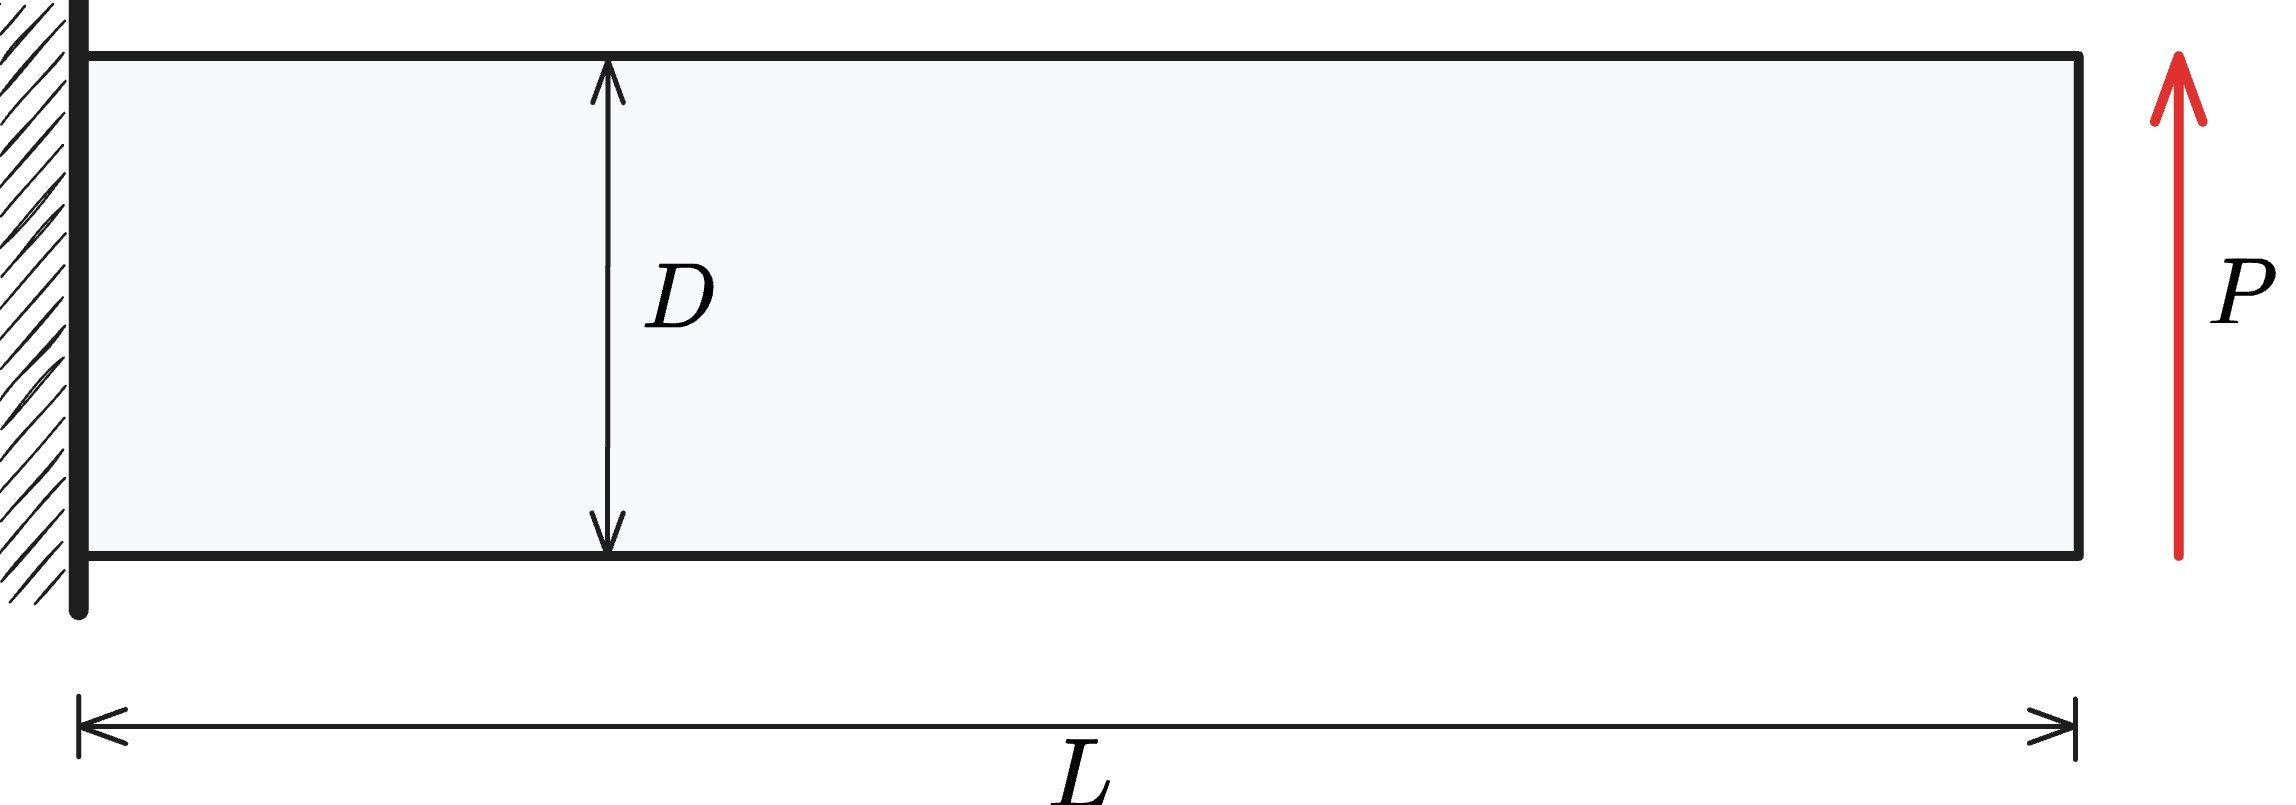
\includegraphics[width=0.7\textwidth]{png/cantilever_model.png}
\caption{Illustration of cantilever beam problem}\label{fg:cantilever_model}
\end{figure}

\begin{figure}[!hp]
\centering
\begin{subcaptiongroup}
\begin{tabular}{c@{\hspace{0pt}}c}
$\Vert \boldsymbol{u} - \boldsymbol{u}_h \Vert_V$ & $\Vert p - p_h \Vert_Q$ \\
\raisebox{-0.8\height}{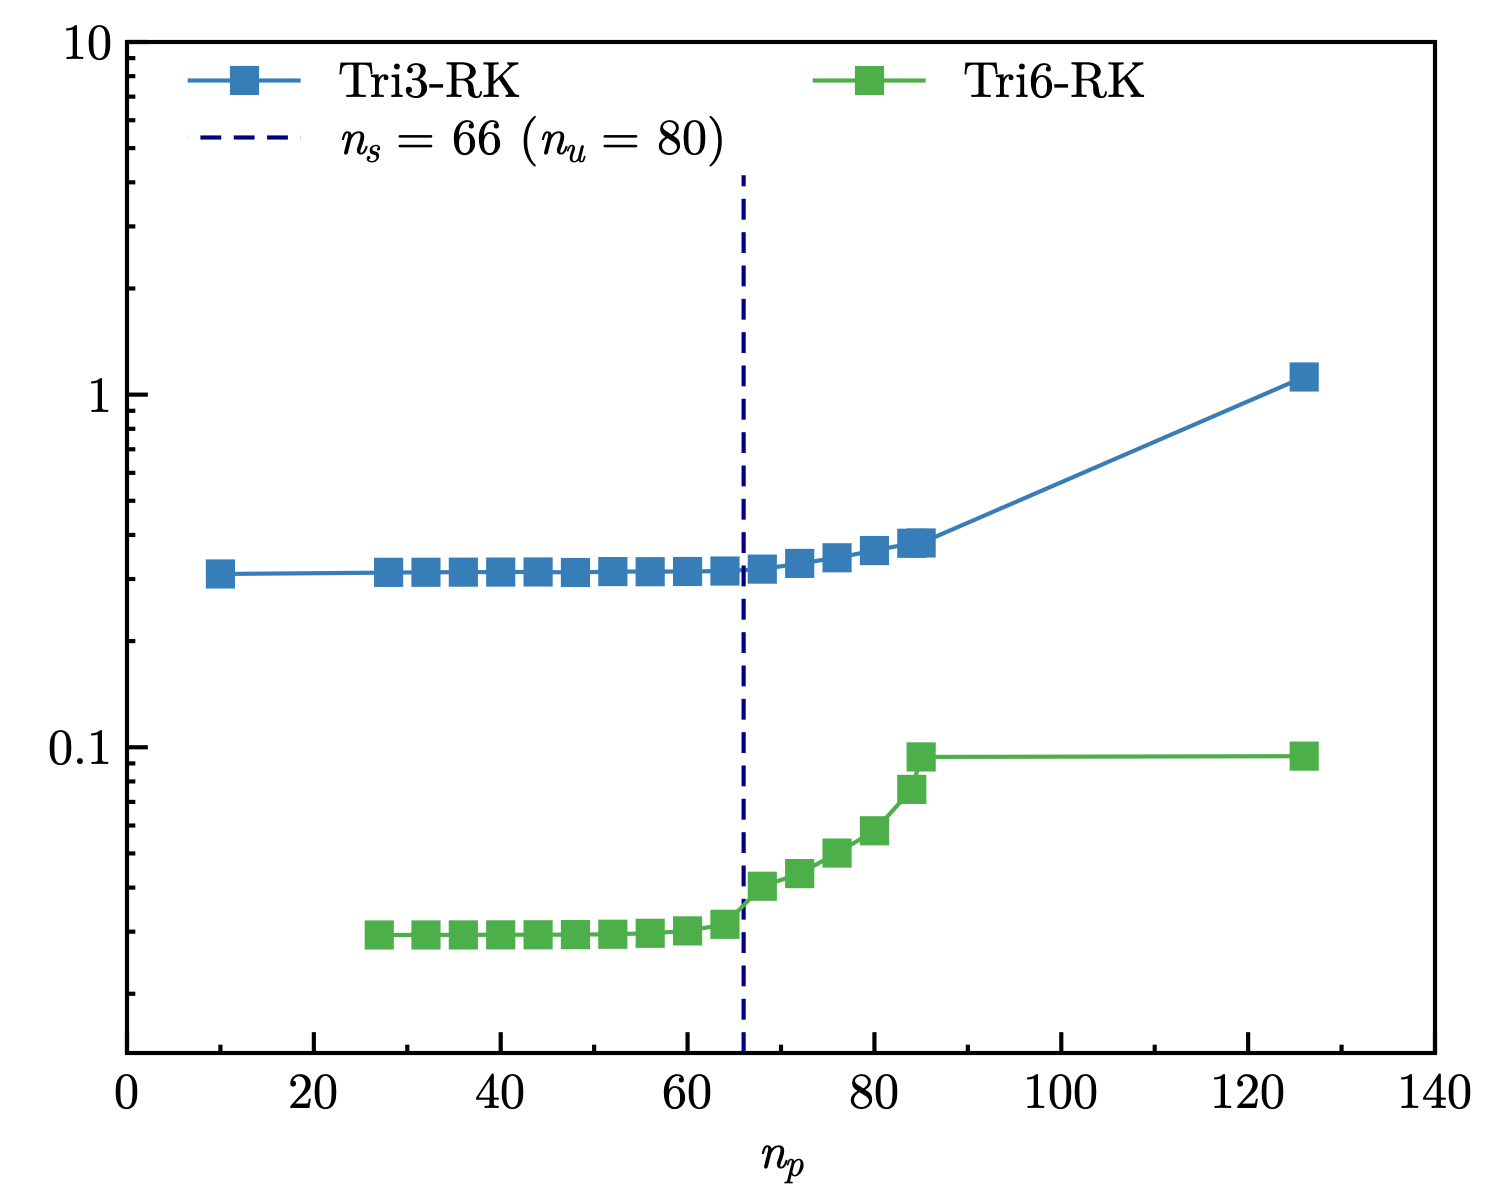
\includegraphics[width=0.48\textwidth]{png/cantilever_tri_Hdev_4.png}}
& \raisebox{-0.8\height}{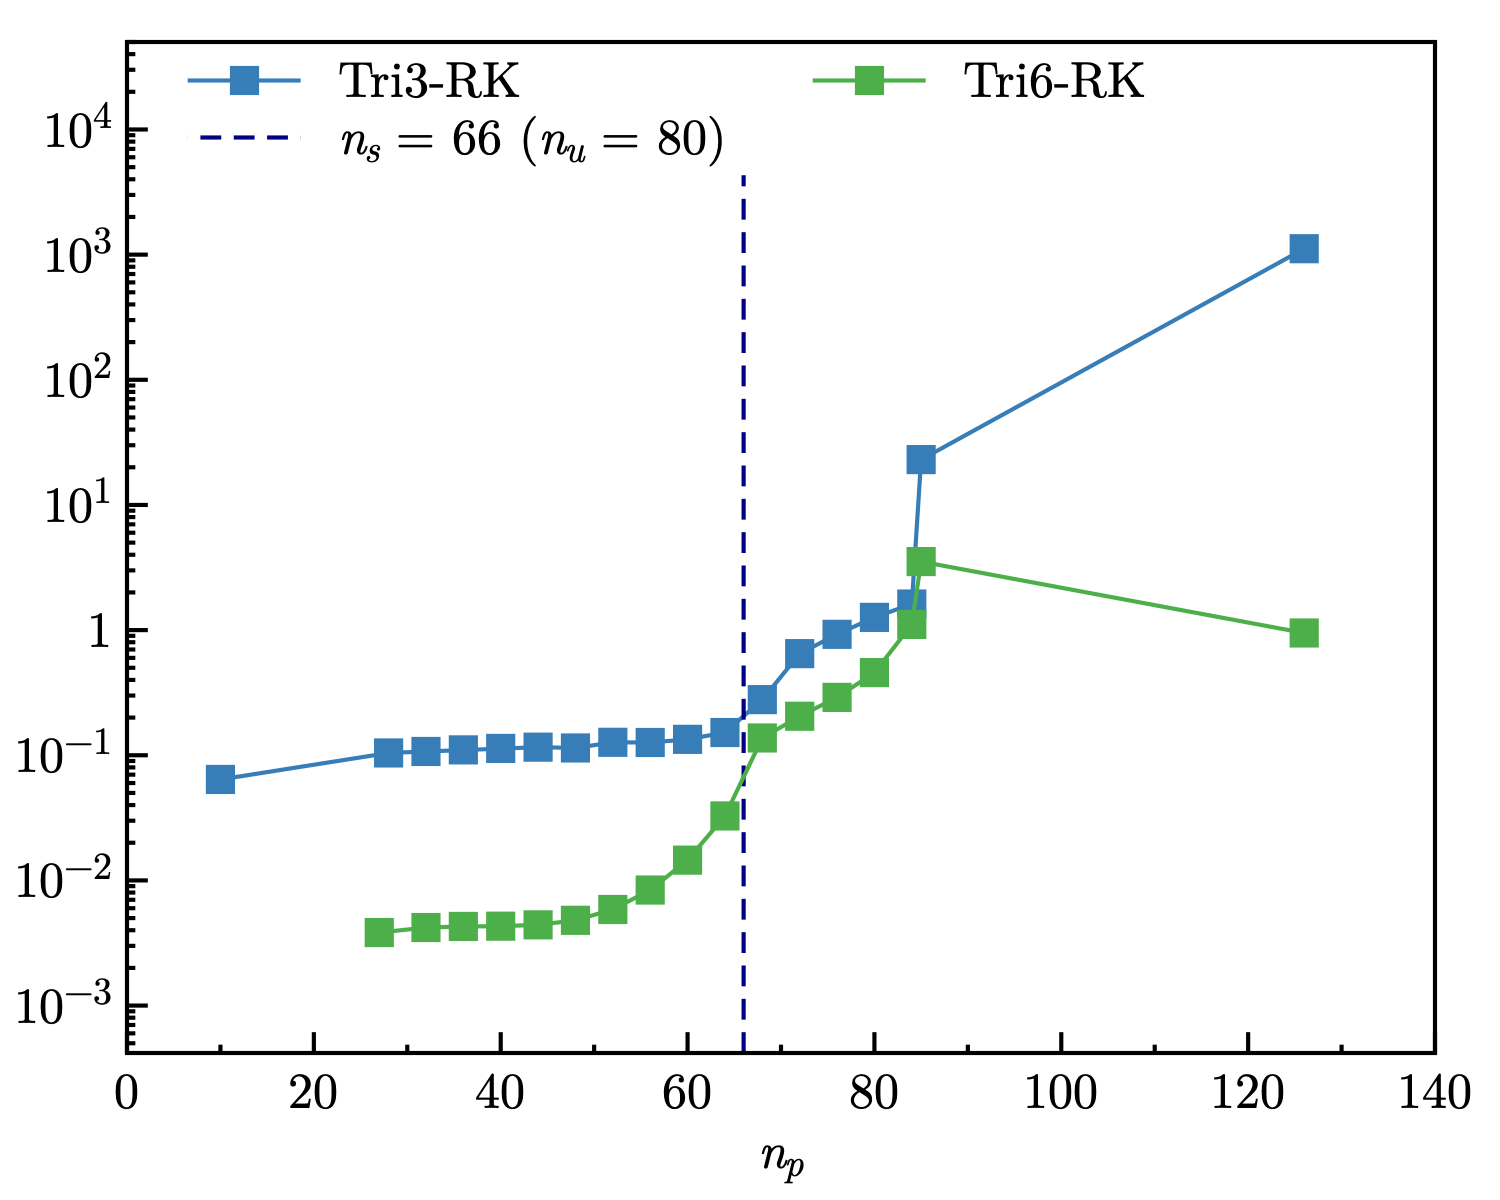
\includegraphics[width=0.48\textwidth]{png/cantilever_tri_L2_p_4.png}} \\
\raisebox{-0.85\height}{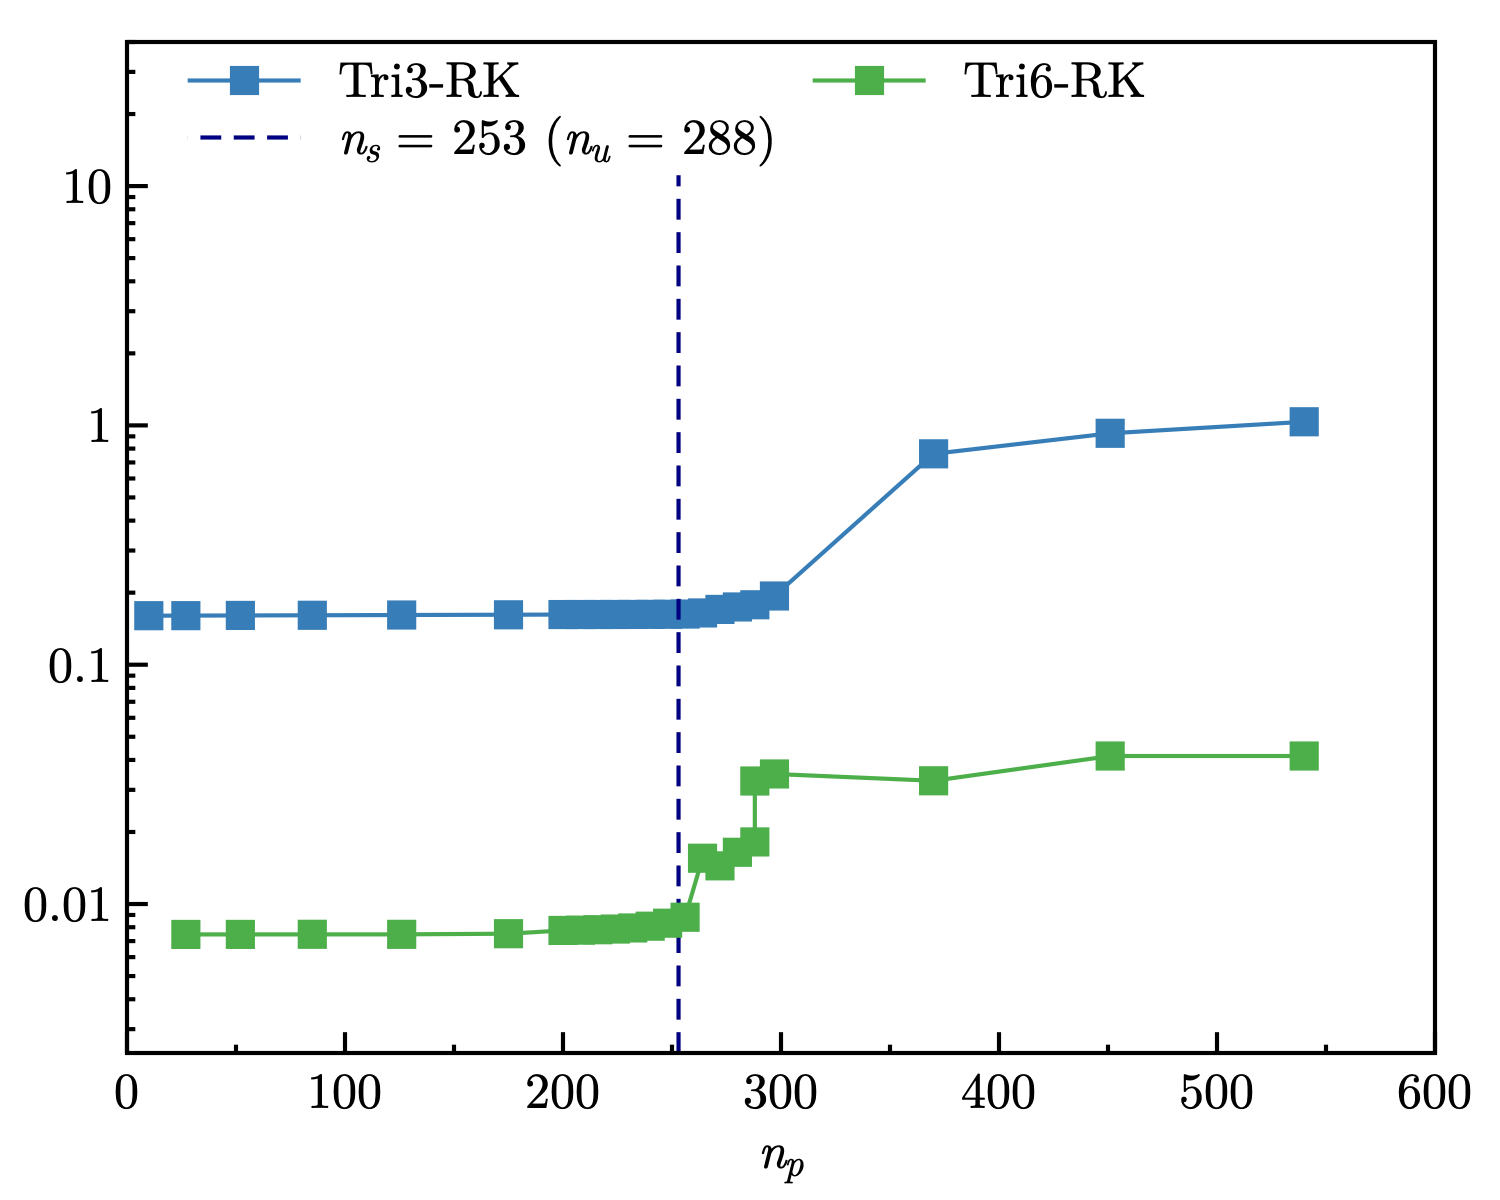
\includegraphics[width=0.48\textwidth]{png/cantilever_tri_Hdev_8.png}}
& \raisebox{-0.85\height}{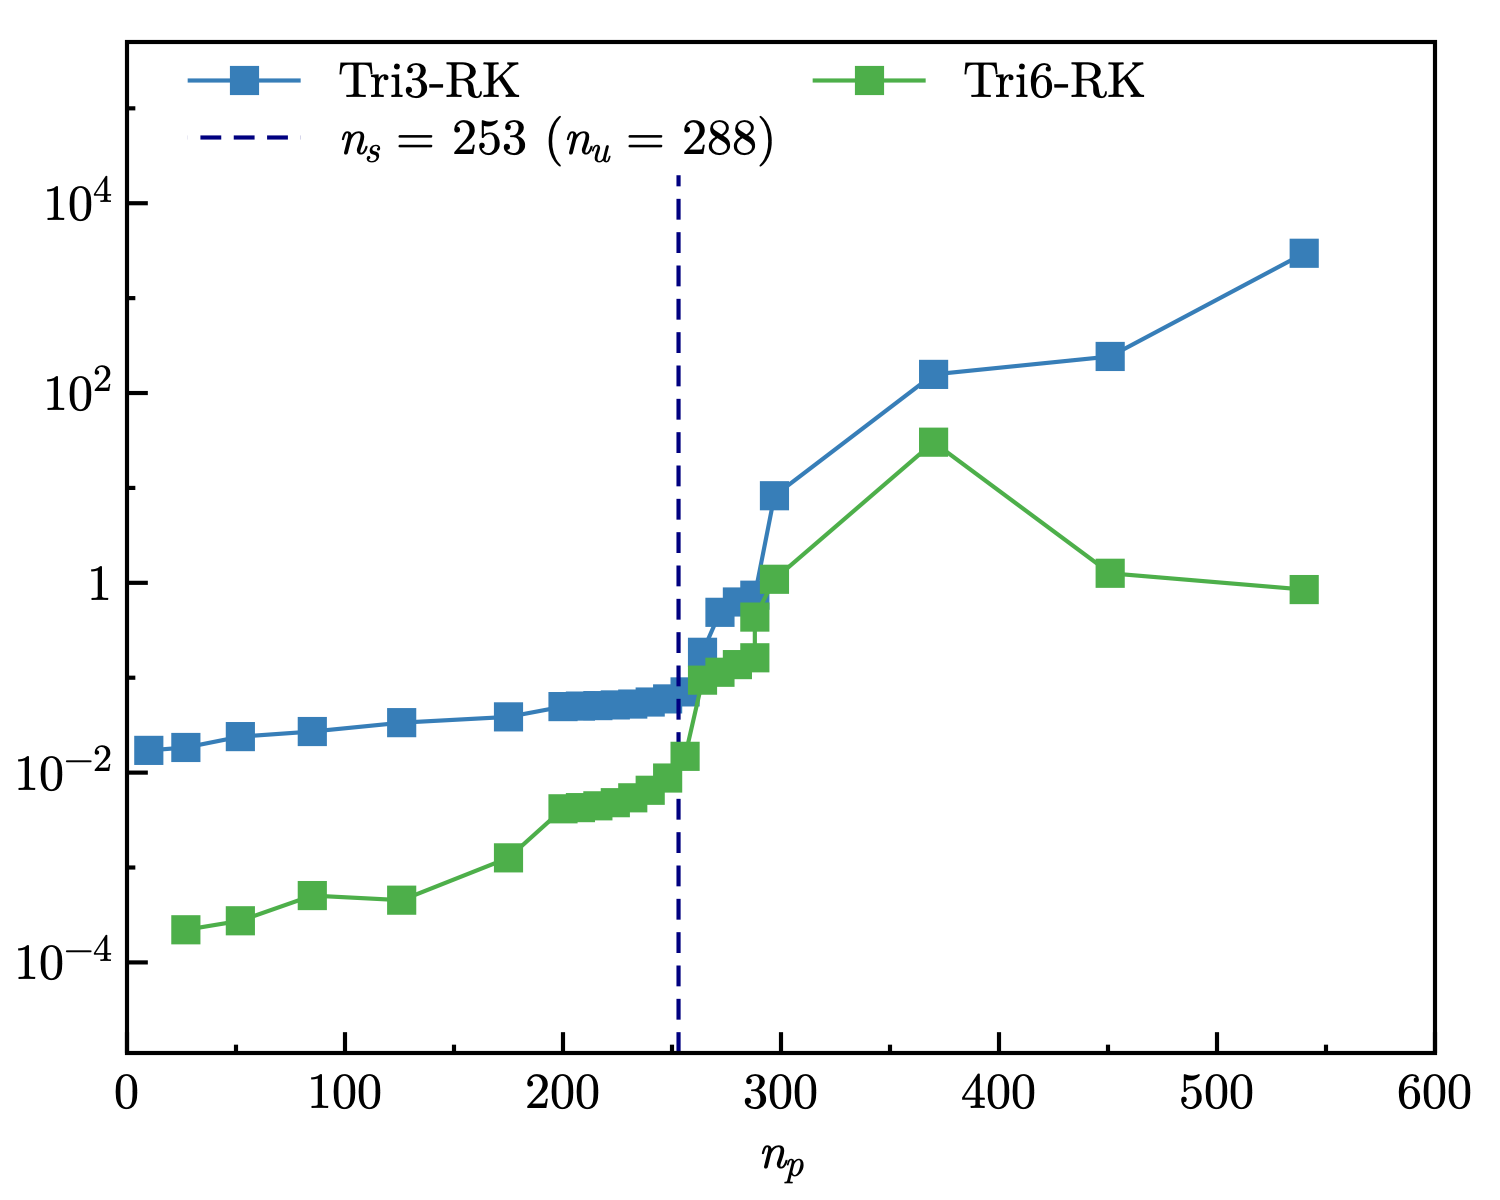
\includegraphics[width=0.48\textwidth]{png/cantilever_tri_L2_p_8.png}} \\
\raisebox{-0.85\height}{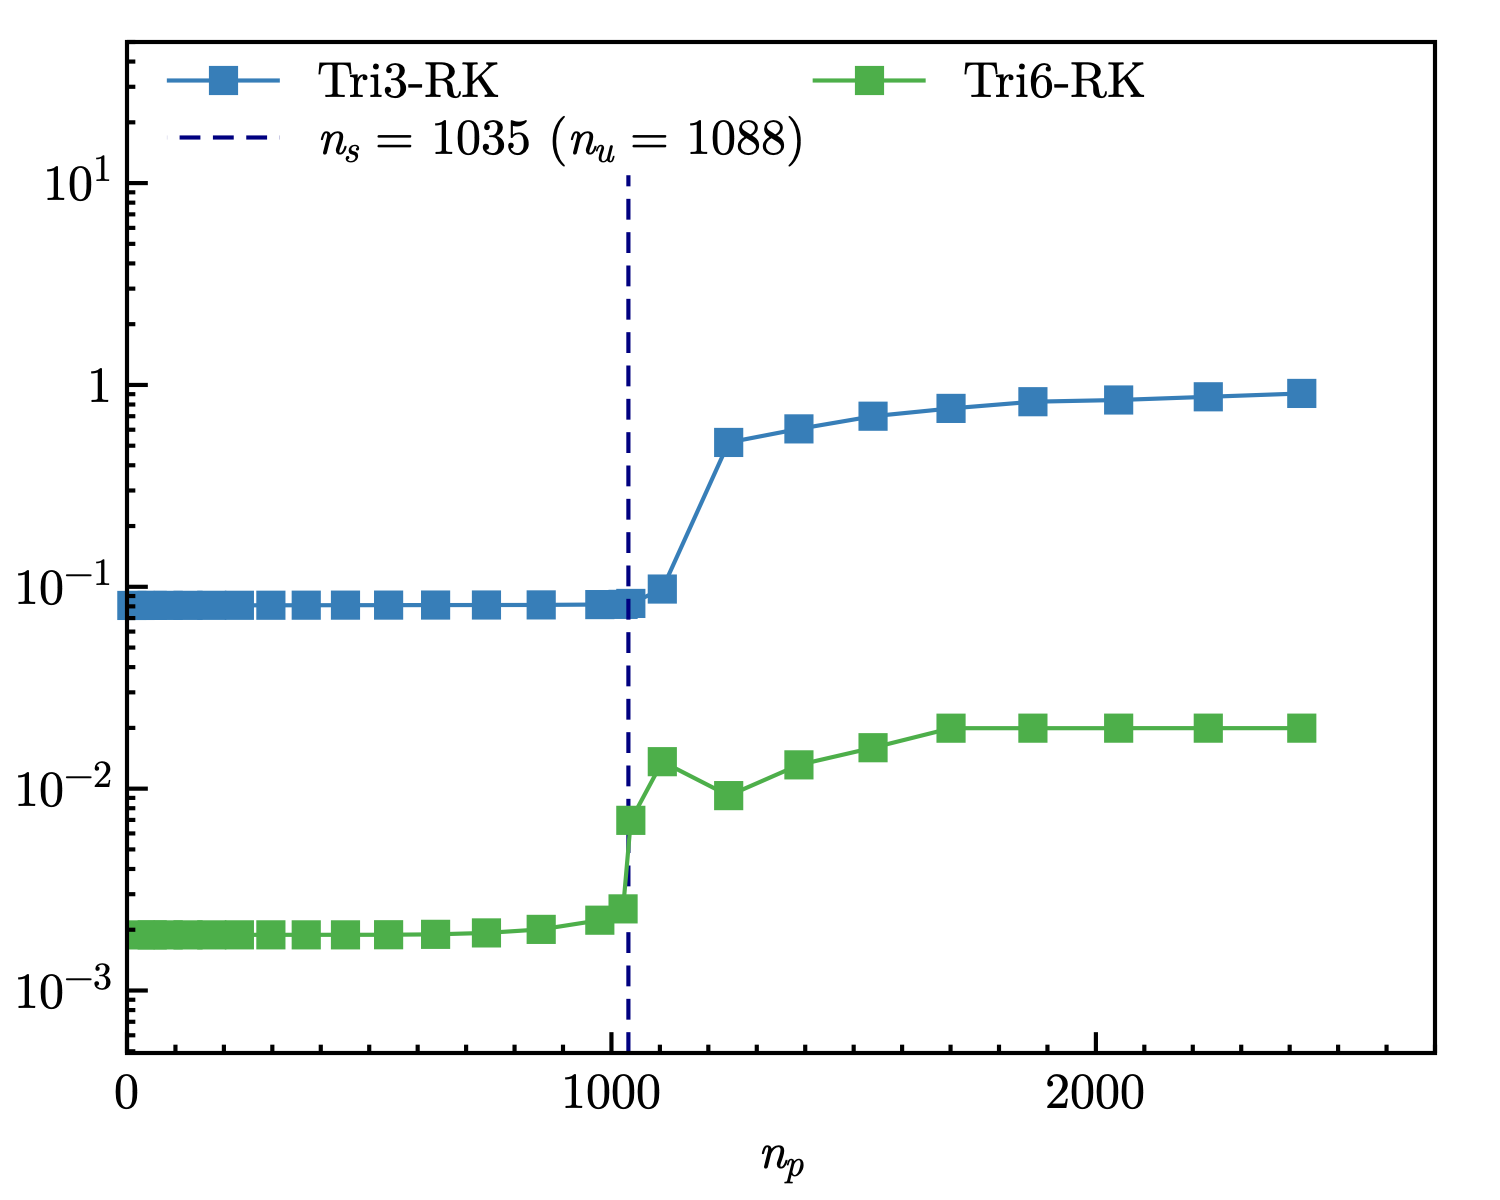
\includegraphics[width=0.48\textwidth]{png/cantilever_tri_Hdev_16.png}}
& \raisebox{-0.85\height}{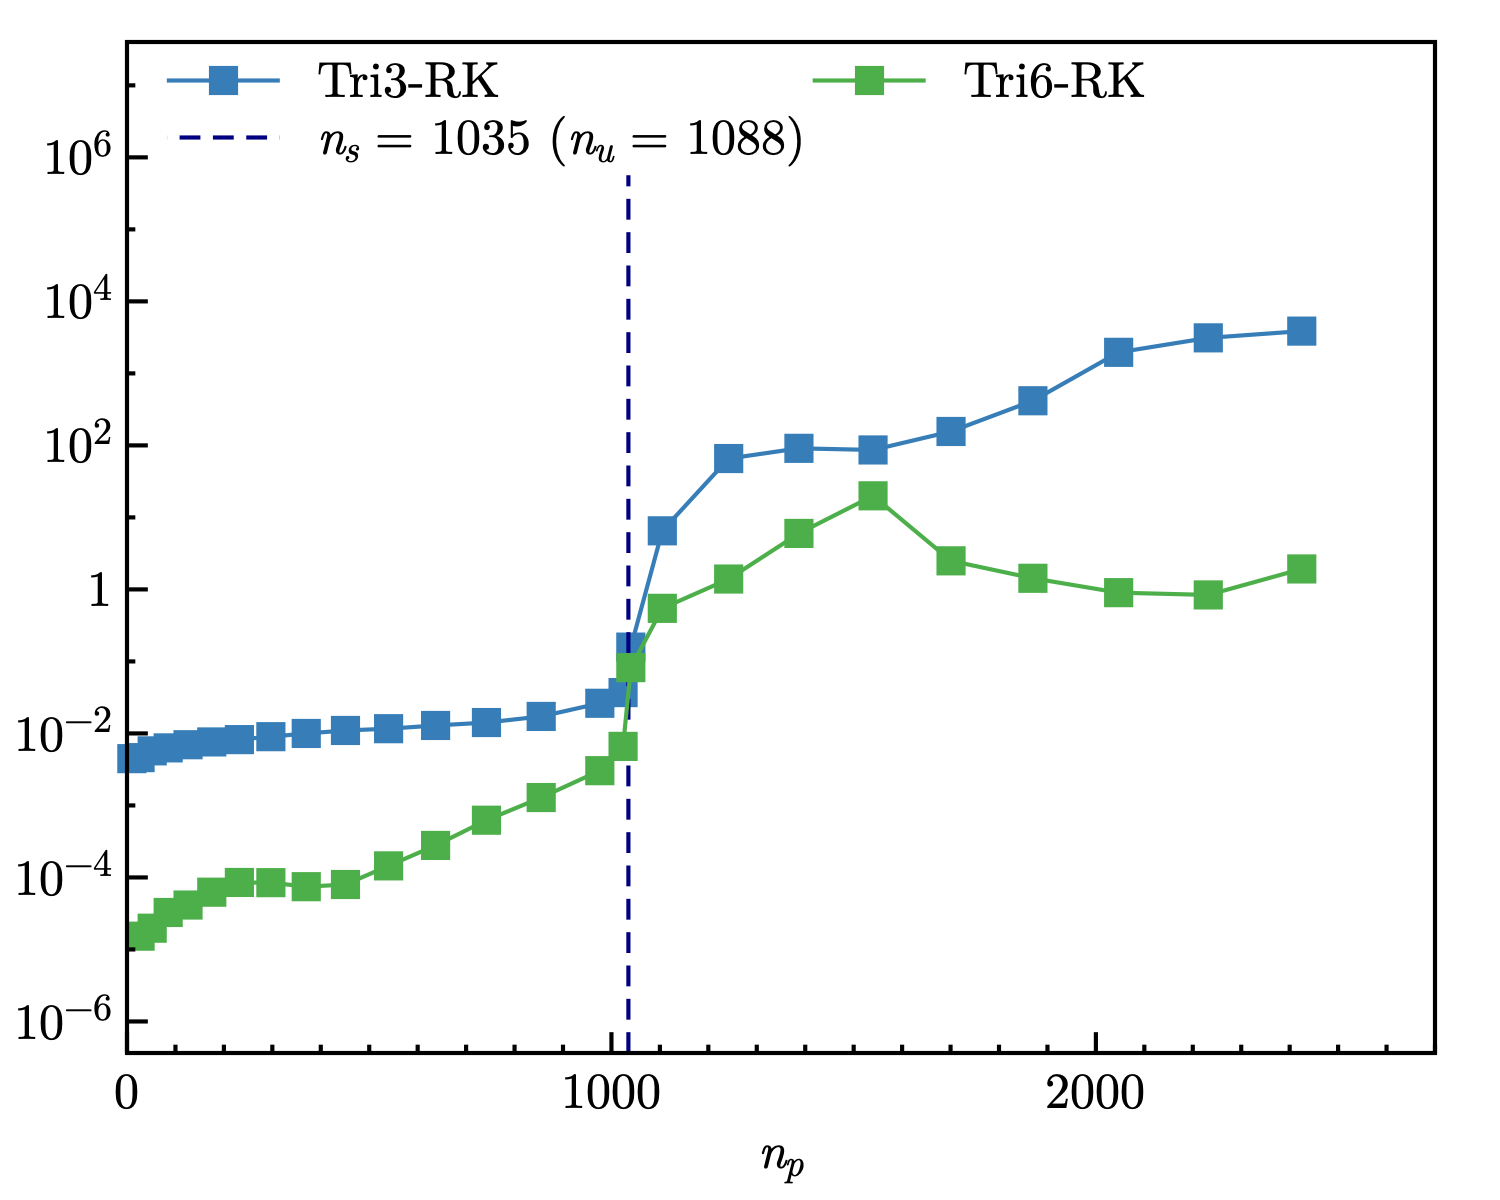
\includegraphics[width=0.48\textwidth]{png/cantilever_tri_L2_p_16.png}} \\
\raisebox{-0.85\height}{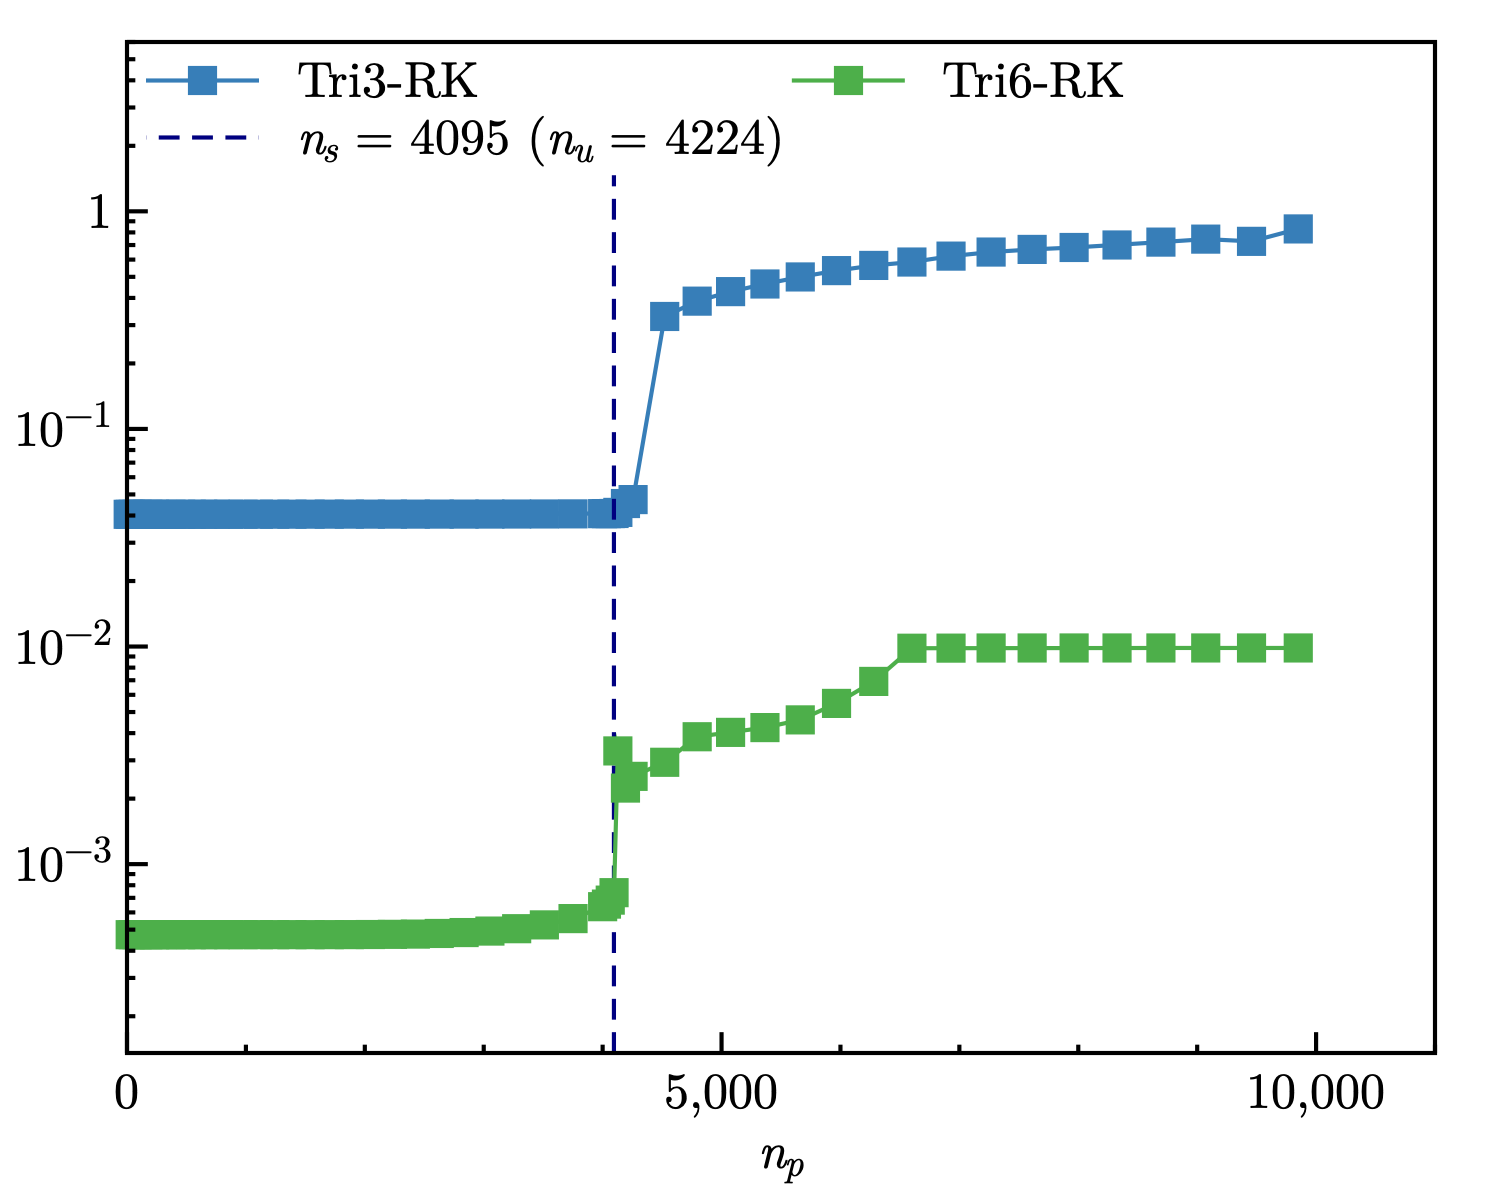
\includegraphics[width=0.48\textwidth]{png/cantilever_tri_Hdev_32.png}}
 & \raisebox{-0.85\height}{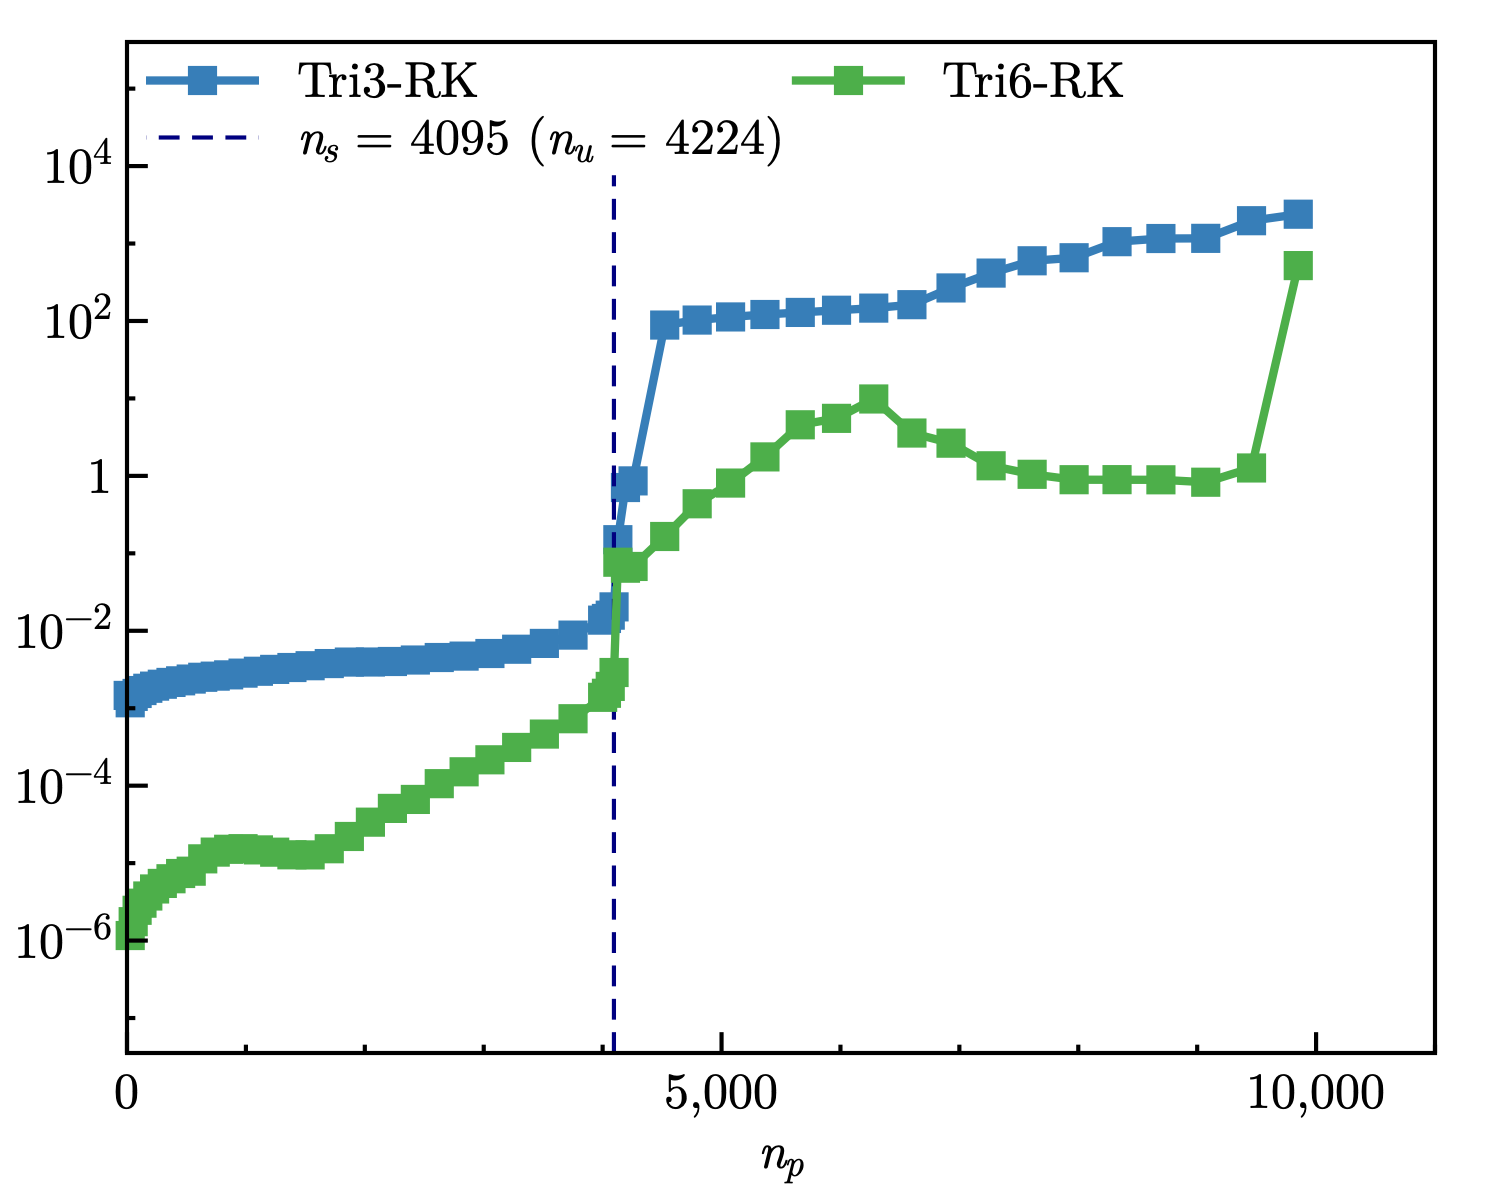
\includegraphics[width=0.48\textwidth]{png/cantilever_tri_L2_p_32.png}} \\
\end{tabular}
\end{subcaptiongroup}
\caption{Strain and pressure errors vs. $n_p$ for cantilever beam problem with triangular elements}\label{fg:cantilever_tri_ns}
\end{figure}

\begin{figure}[!hp]
\centering
\begin{subcaptiongroup}
\begin{tabular}{c@{\hspace{0pt}}c}
$\Vert \boldsymbol{u} - \boldsymbol{u}_h \Vert_V$ & $\Vert p - p_h \Vert_Q$ \\
\raisebox{-0.8\height}{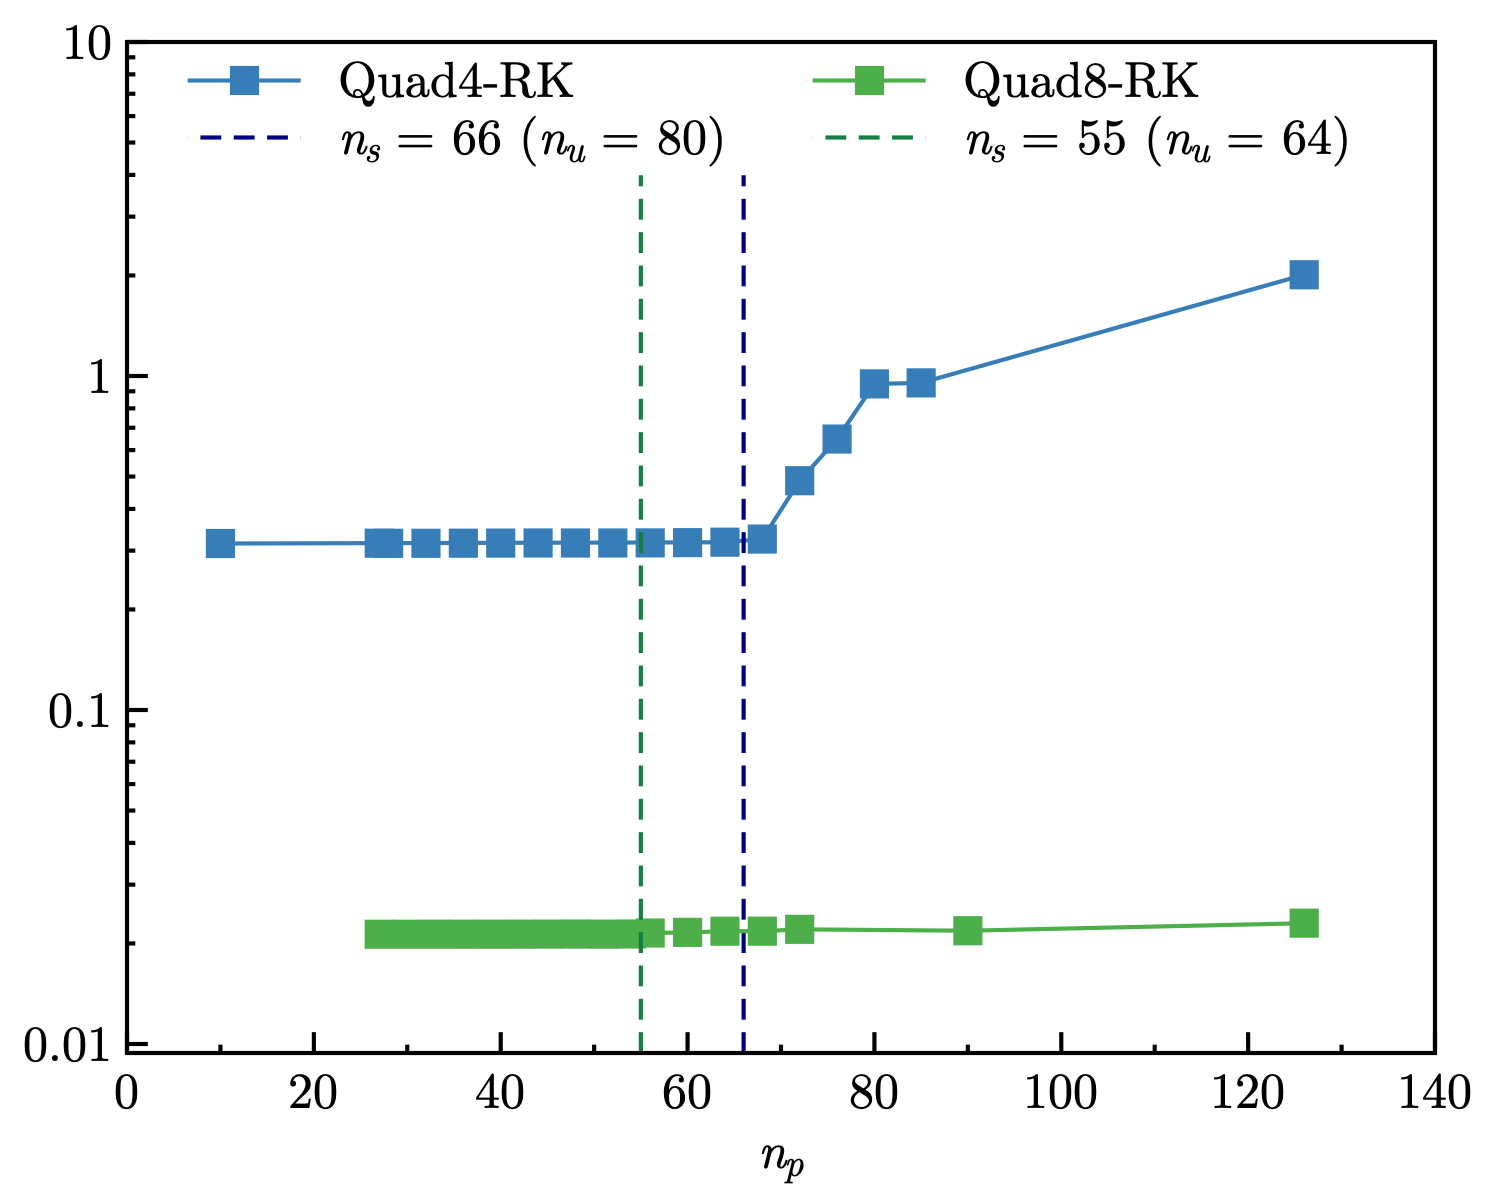
\includegraphics[width=0.48\textwidth]{png/cantilever_Hdev_4.png}}
& \raisebox{-0.8\height}{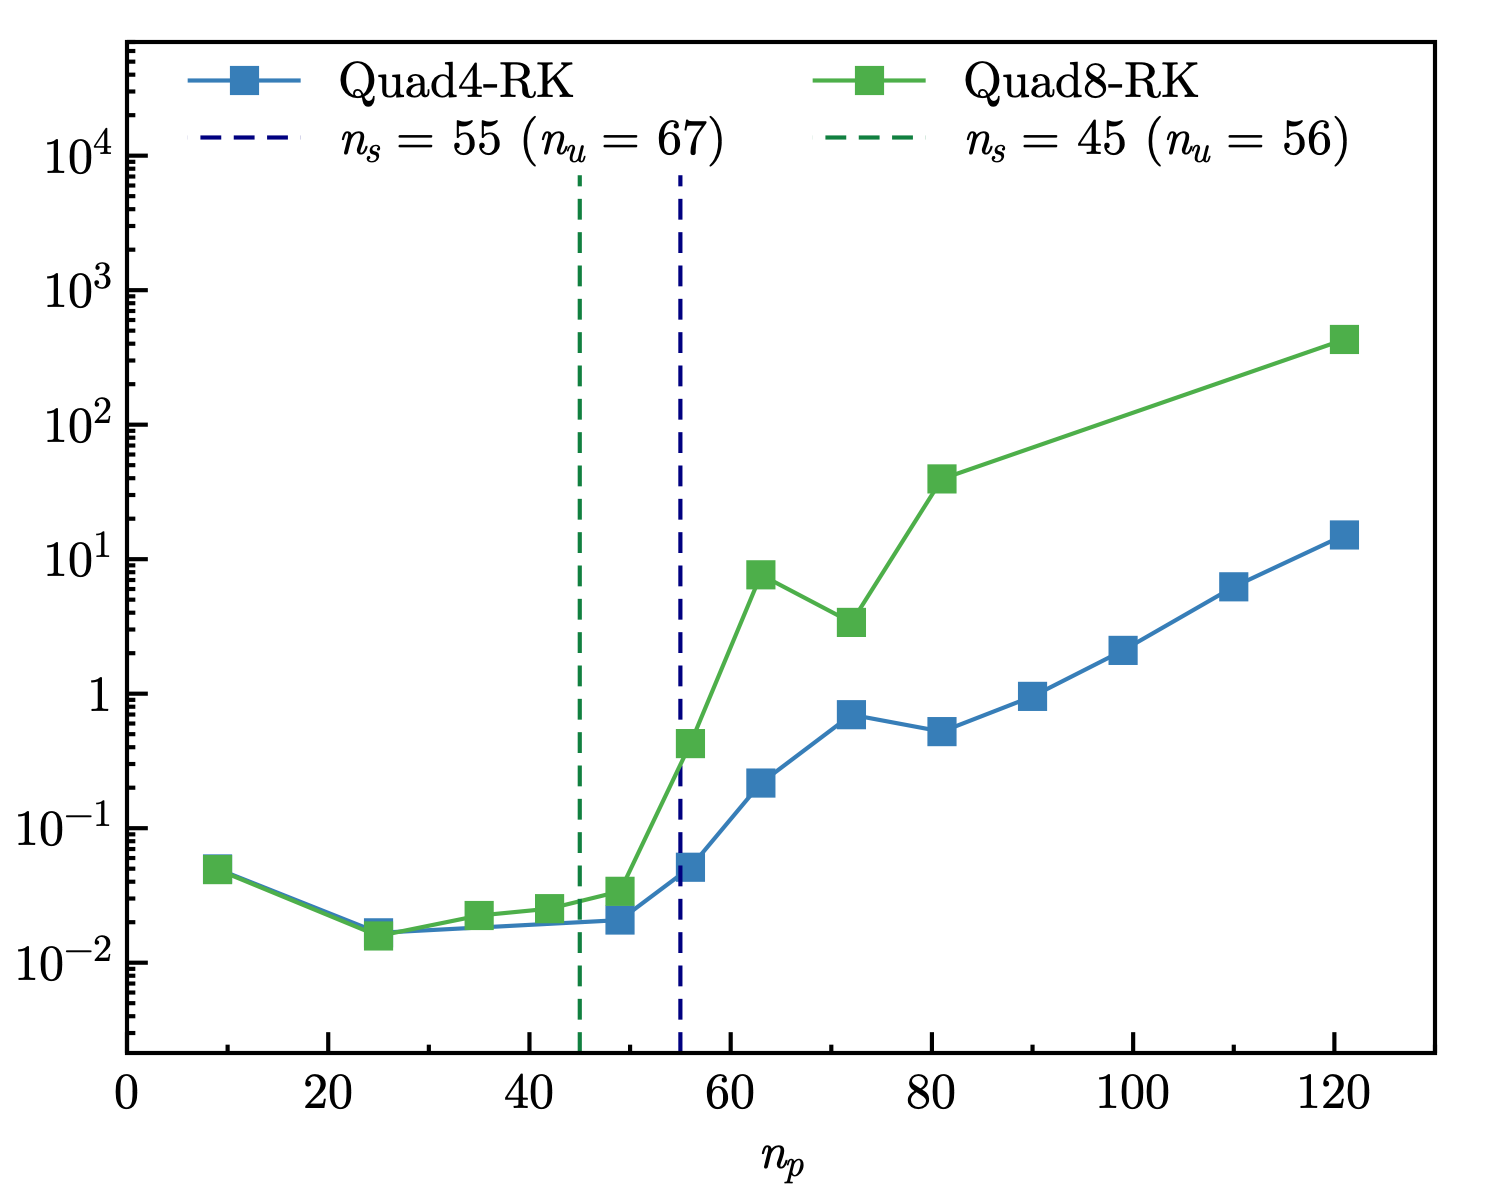
\includegraphics[width=0.48\textwidth]{png/cantilever_L2_p_4.png}} \\
\raisebox{-0.85\height}{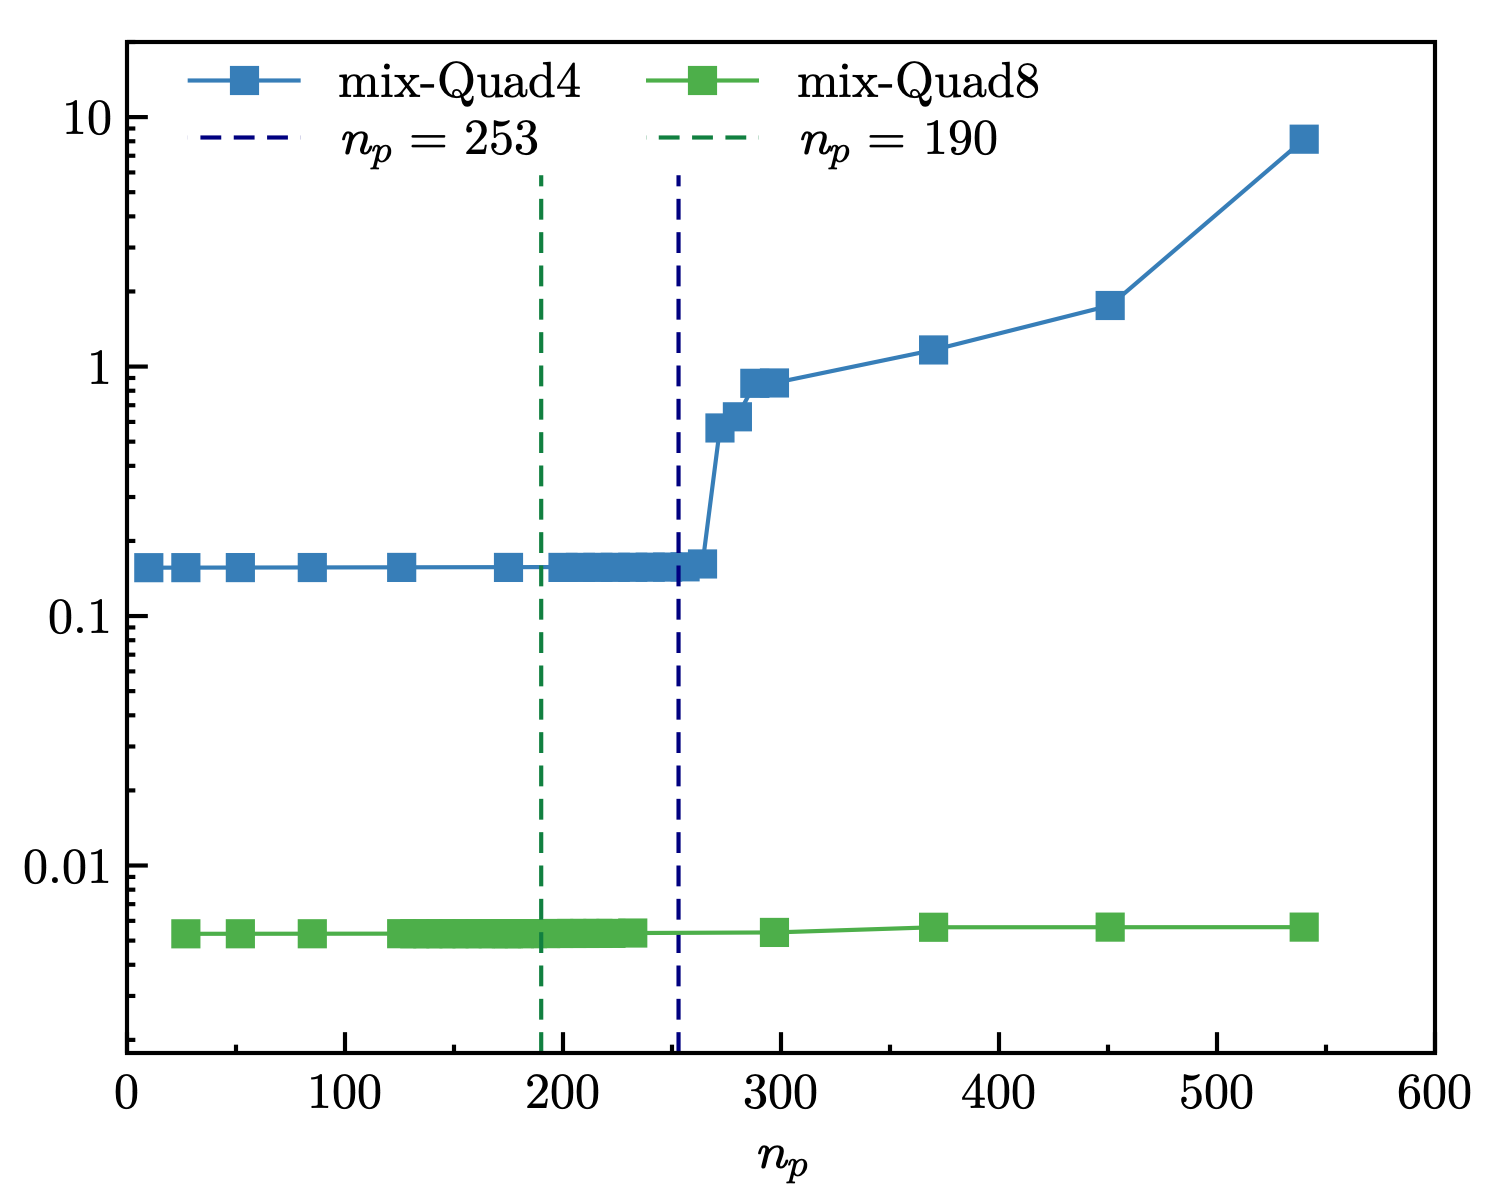
\includegraphics[width=0.48\textwidth]{png/cantilever_Hdev_8.png}}
& \raisebox{-0.85\height}{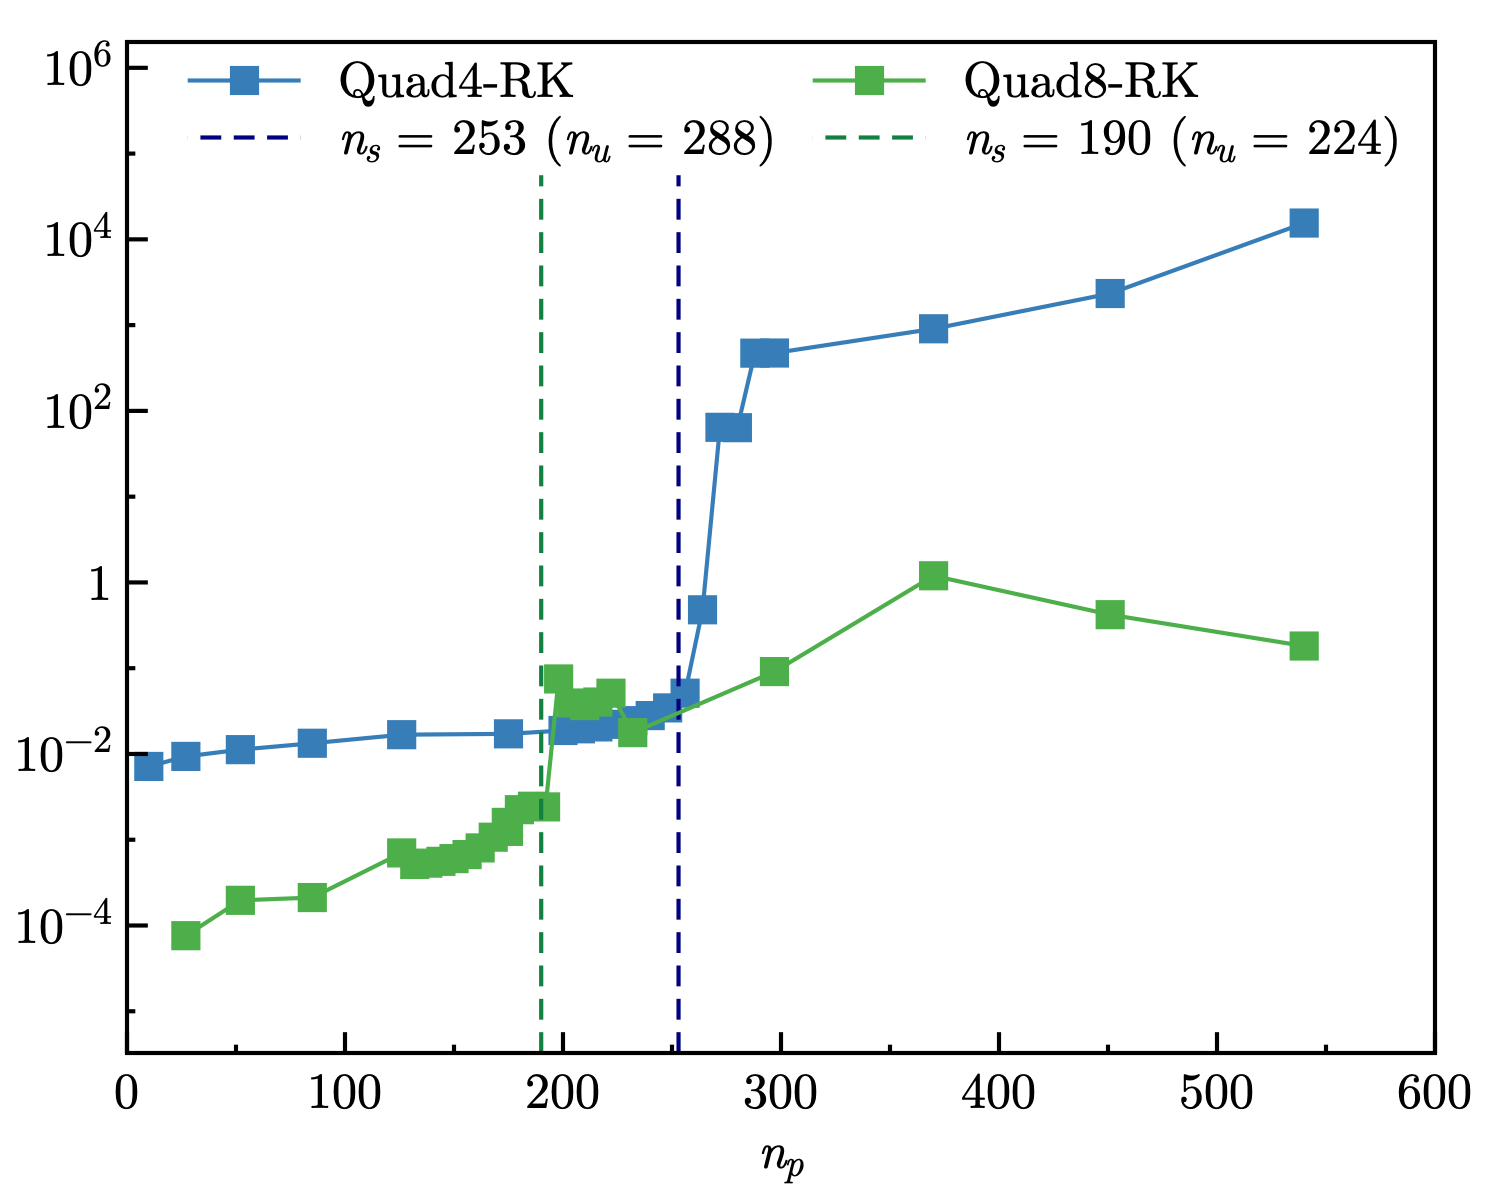
\includegraphics[width=0.48\textwidth]{png/cantilever_L2_p_8.png}} \\
\raisebox{-0.85\height}{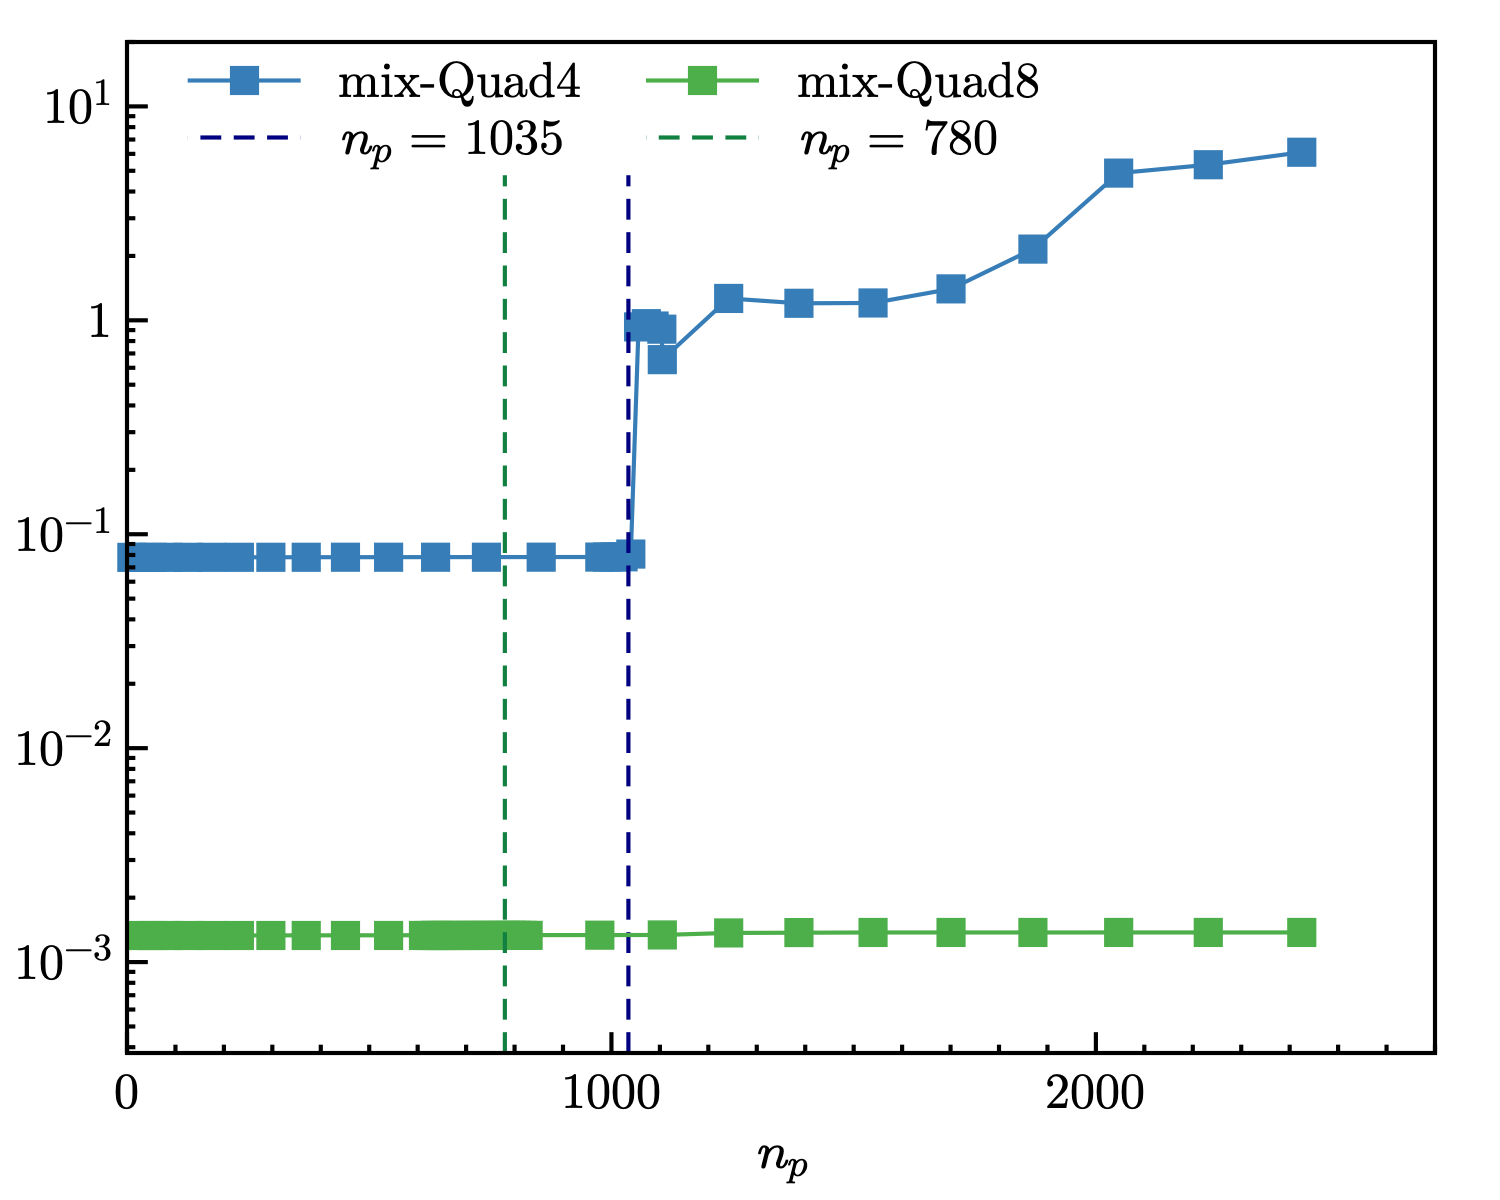
\includegraphics[width=0.48\textwidth]{png/cantilever_Hdev_16.png}}
& \raisebox{-0.85\height}{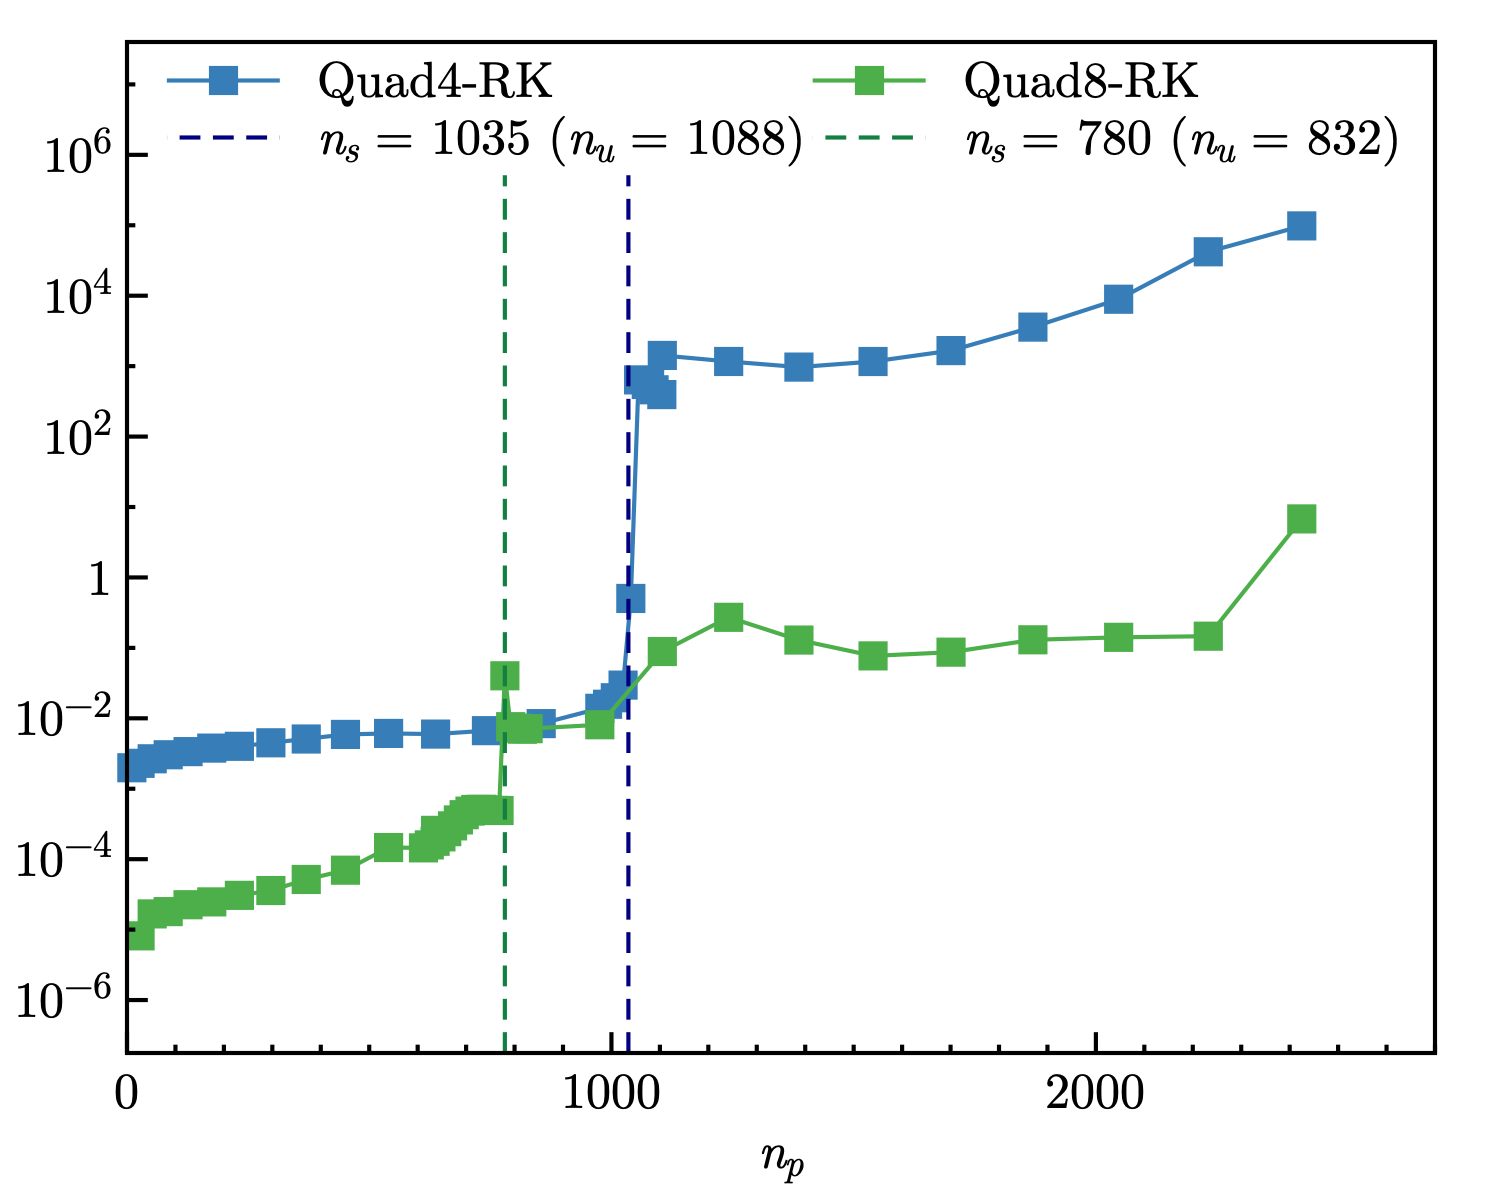
\includegraphics[width=0.48\textwidth]{png/cantilever_L2_p_16.png}} \\
\raisebox{-0.85\height}{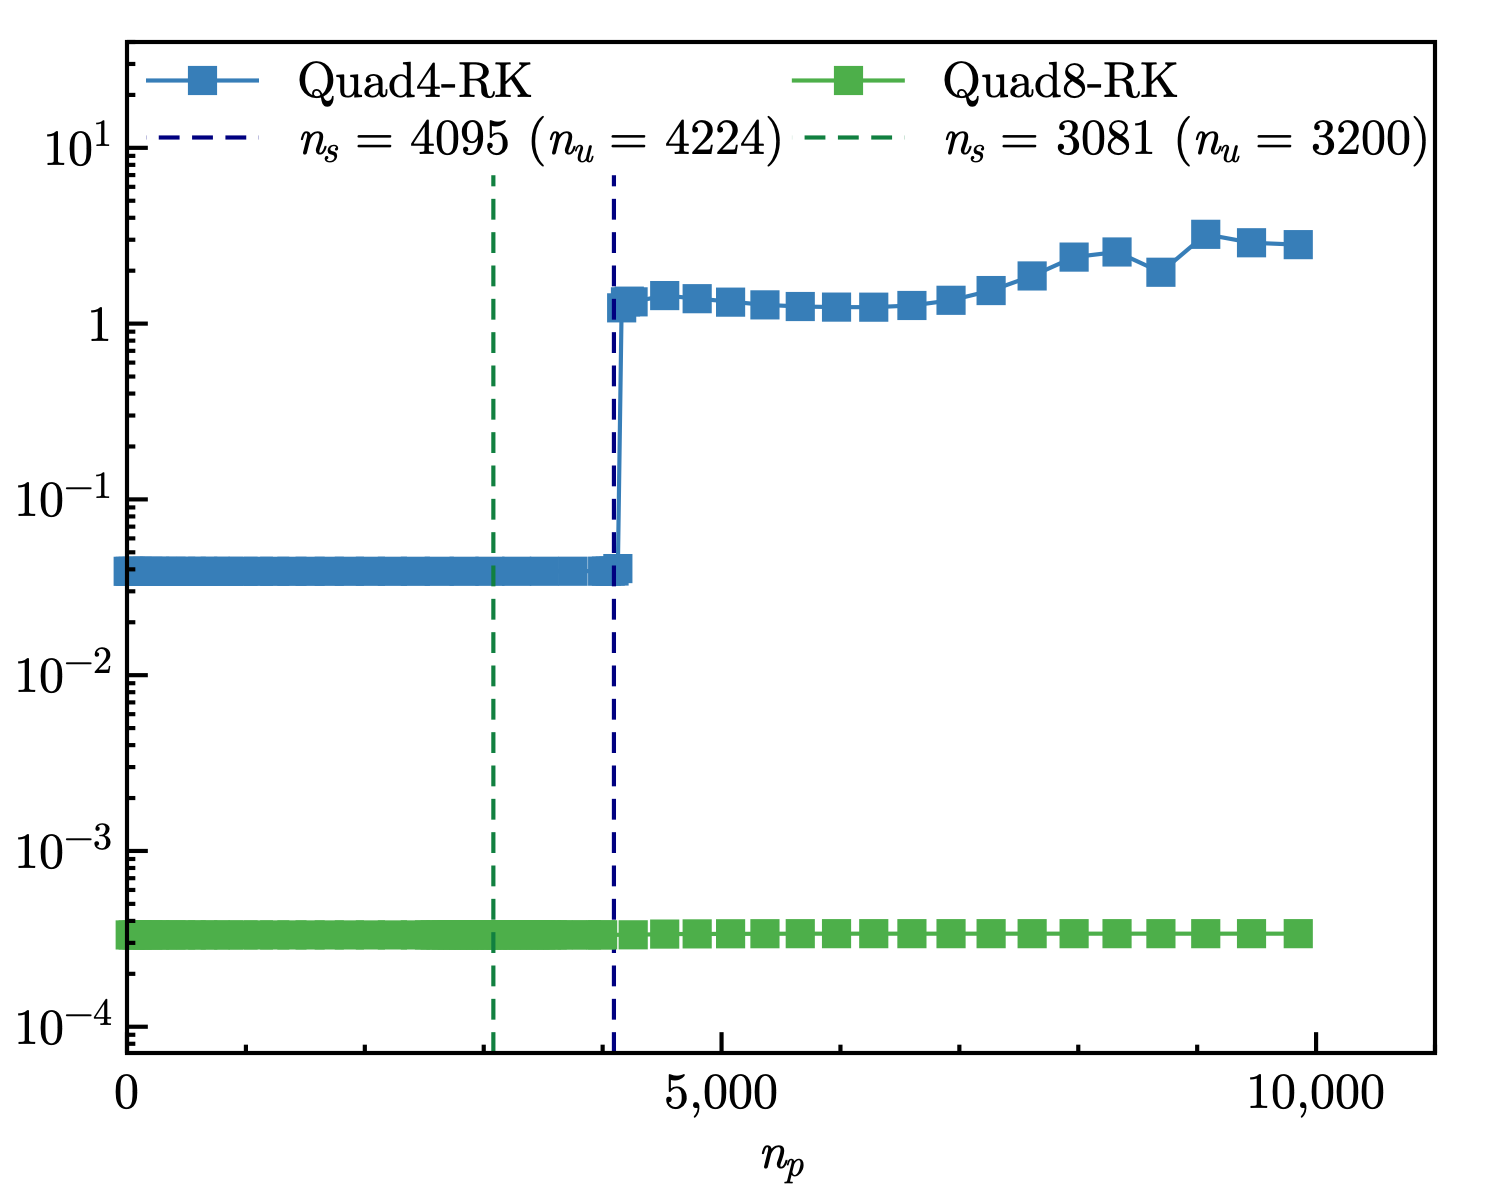
\includegraphics[width=0.48\textwidth]{png/cantilever_Hdev_32.png}}
 & \raisebox{-0.85\height}{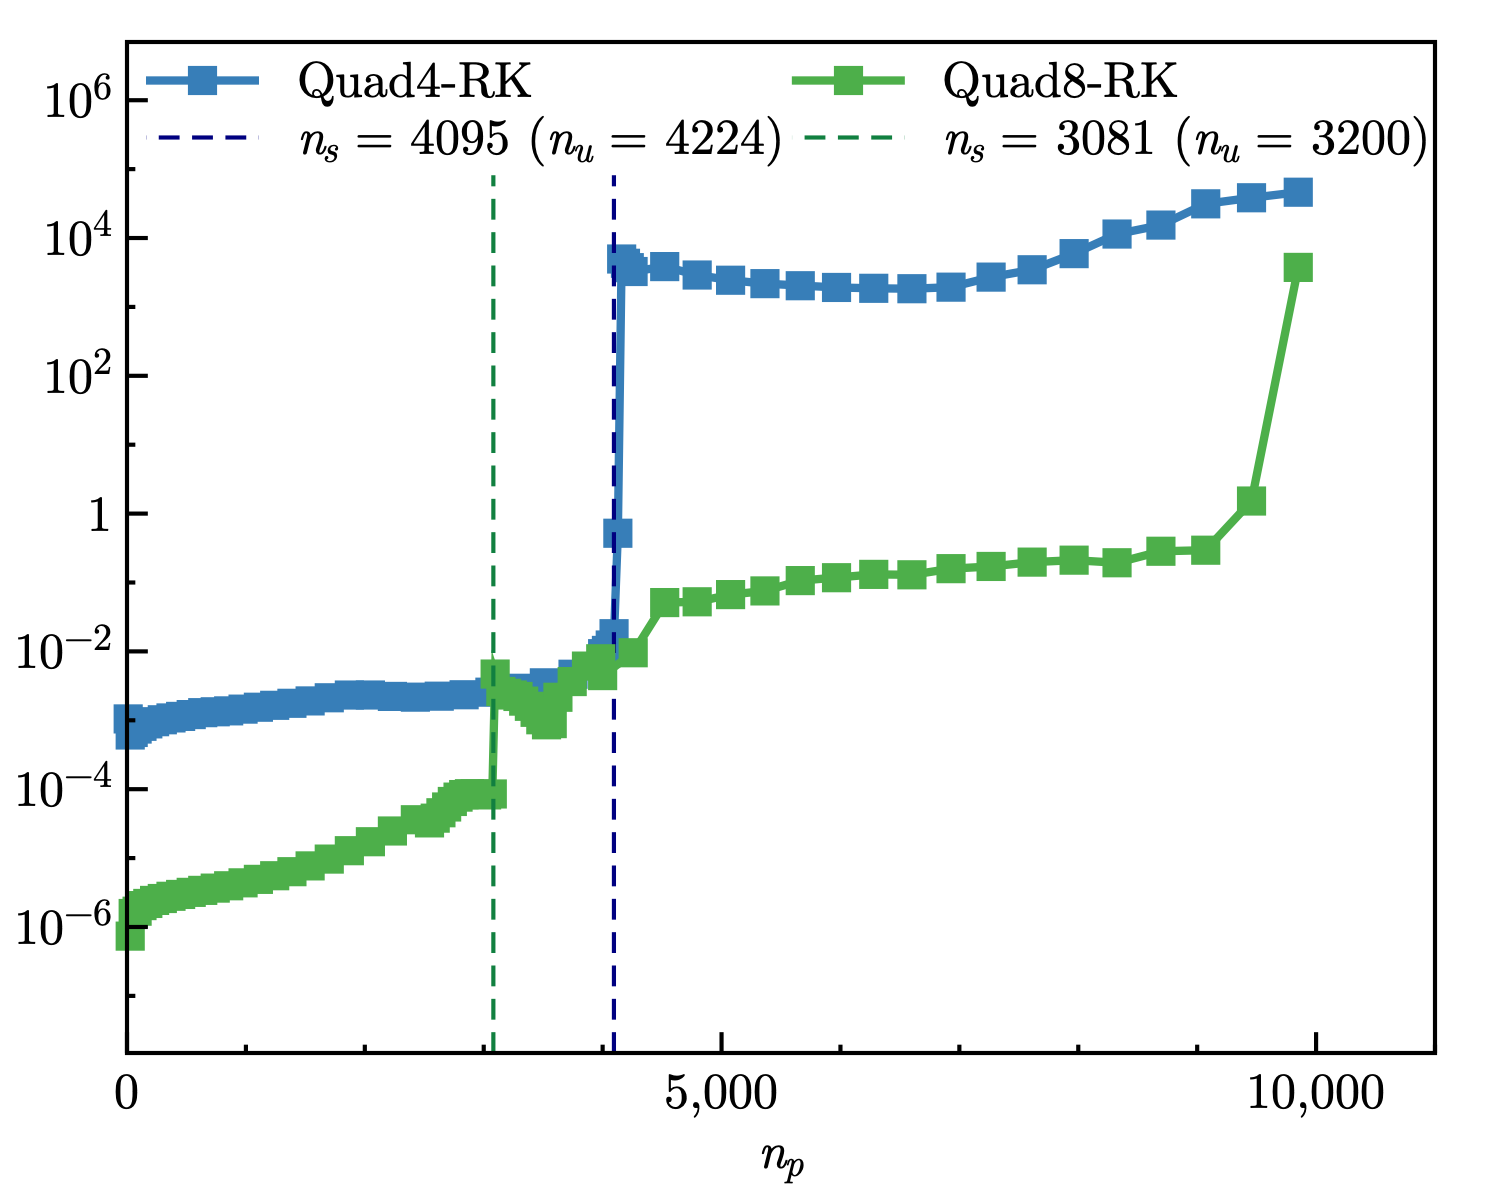
\includegraphics[width=0.48\textwidth]{png/cantilever_L2_p_32.png}} \\
\end{tabular}
\end{subcaptiongroup}
\caption{Strain and pressure errors vs. $n_p$ for cantilever beam problem with quadrilateral elements}\label{fg:cantilever_ns}
\end{figure}

In this problem, the Tri3, Quad4 elements with $16\times 4$, $32\times 8$, $64\times 16$, $128\times 32$ grids, and Tri6, Quad8 elements with $8\times 2$, $16\times 4$, $32\times 8$, $64\times 16$ grids are employed for displacement discretization. The pressure is discretized by linear and quadratic meshfree approximations with 1.5 and 2.5 characterized support sizes respectively.
The strain and pressure errors with respect to pressure nodes $n_p$ are displayed in Figures \ref{fg:cantilever_tri_ns}, \ref{fg:cantilever_ns}, where, to avoid the interpolation error, the pressure nodes are uniformly distributed independent with displacement nodes by the same way in Section \ref{subsec:optimal_constraint_ratio}. 
The vertical dashed lines stand for the stabilized number $n_s$.
The figures imply that all pressure errors immediately increase when their constraint ratios are out of the optimal range,
and quadratic elements still have better results than linear elements.
As $n_p$ becomes very small, the pressure errors do not increase.
This is because the pressure error estimator in Eq. \eqref{p_estimator} is primarily controlled by the strain error and the inf-sup value $\beta$.
The exact pressure solution in Eq. \eqref{cantilever_stress} is only a second-order polynomial. As a result, the pressure interpolation error in Eq. \eqref{p_estimator} is either very small or nonexistent.
For the strain error, the Quad8--RK method shows stable results regardless of whether the constraint ratio is in the optimal range.
This may be due to the fact that the Quad8 element with a regular mesh satisfies the relationship of Eq. \eqref{interp_error_0}.
In this context, the strain error of Eq. \eqref{u_estimator} is independent of the inf-sup value $\beta$ and remains at a low level.

Additionally, a non-uniform discretization version of the study on strain and pressure errors with respect to $n_p$ is conducted shown in Figure \ref{fg:cantilever_irregular_mesh}.
To avoid the influence of the pressure interpolation error, the pressure nodes are still uniformly distributed, independent of the displacement nodes.
The results in Figure \ref{fg:cantilever_ns_irregular} show that the pressure errors of linear approximations, Tri3--RK and Quad4--RK, immediately increase when their constraint ratios are outside the optimal range.
The quadratic approximations, Tri6--RK and Quad8--RK, demonstrate better performance in resisting volumetric locking.
In this case, the increase in pressure error has a gentler slope when the number of pressure nodes exceeds $n_s$.

\begin{figure}[H]
\centering
\begin{subcaptiongroup}
\parbox[b]{0.6\textwidth}{
    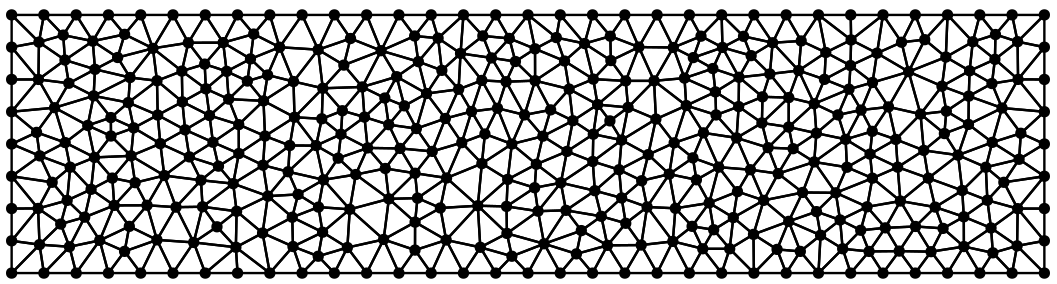
\includegraphics[width=0.6\textwidth]{png/cantilever_tri3_irregular_385.png}
    \caption{Tri3--RK with $n_u=376$}
}
\parbox[b]{0.6\textwidth}{
    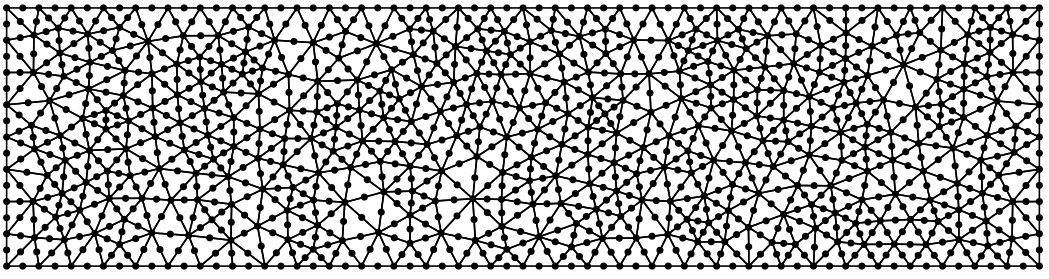
\includegraphics[width=0.6\textwidth]{png/cantilever_tri6_irregular_1457.png}
    \caption{Tri6--RK with $n_u=1440$}
}
\parbox[b]{0.6\textwidth}{
    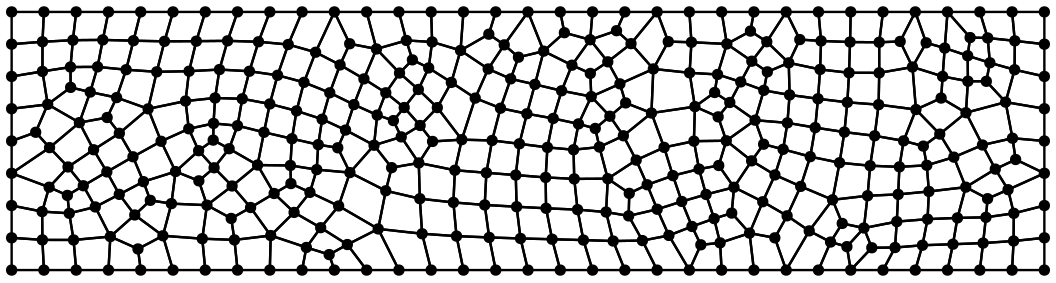
\includegraphics[width=0.6\textwidth]{png/cantilever_quad4_irregular_367.png}
    \caption{Quad4--RK with $n_u=358$}
}
\parbox[b]{0.6\textwidth}{
    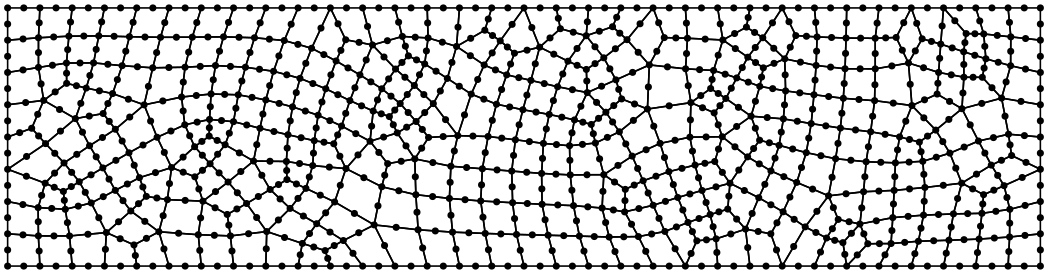
\includegraphics[width=0.6\textwidth]{png/cantilever_quad8_irregular_1059.png}
    \caption{Quad8--RK with $n_u=1042$}
}
\end{subcaptiongroup}
\caption{Non--uniform discretizations for cantilever beam problem}\label{fg:cantilever_irregular_mesh}
\end{figure}

\begin{figure}[!hp]
\centering
\begin{subcaptiongroup}
\begin{tabular}{c@{\hspace{0pt}}c}
$\Vert \boldsymbol{u} - \boldsymbol{u}_h \Vert_V$ & $\Vert p - p_h \Vert_Q$ \\
\raisebox{-0.8\height}{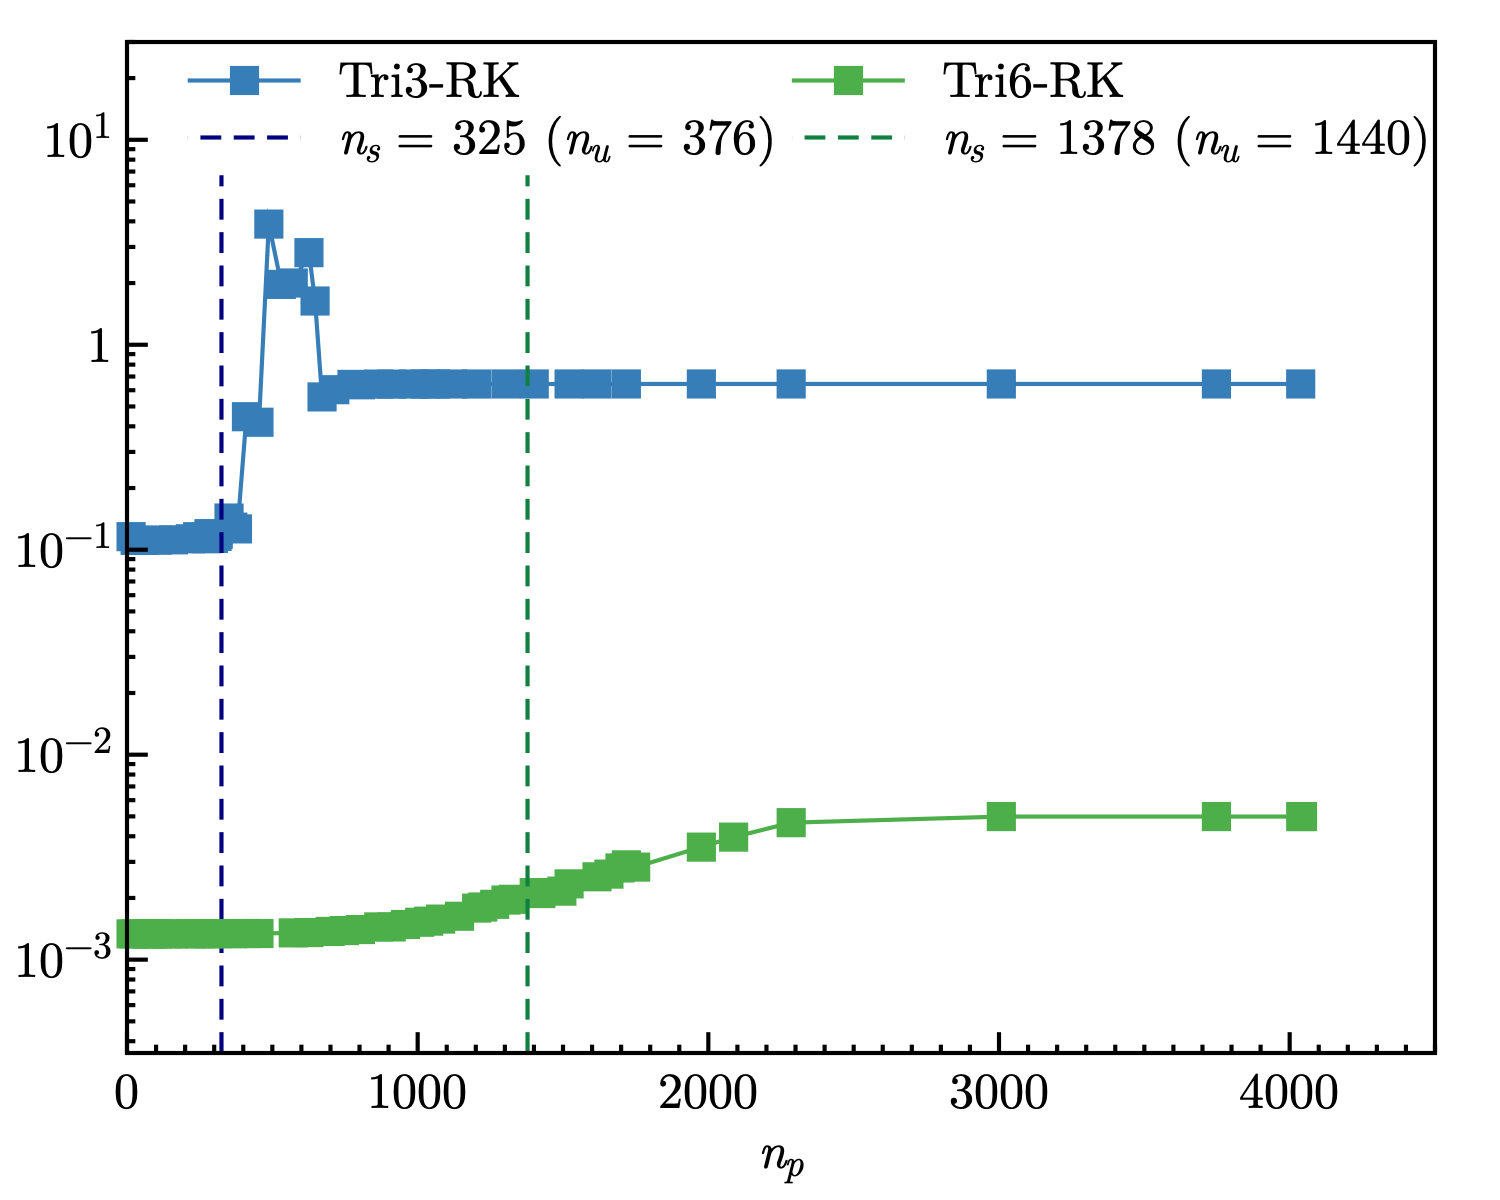
\includegraphics[width=0.48\textwidth]{png/cantilever_tri_irregular_Hdev.png}}
& \raisebox{-0.8\height}{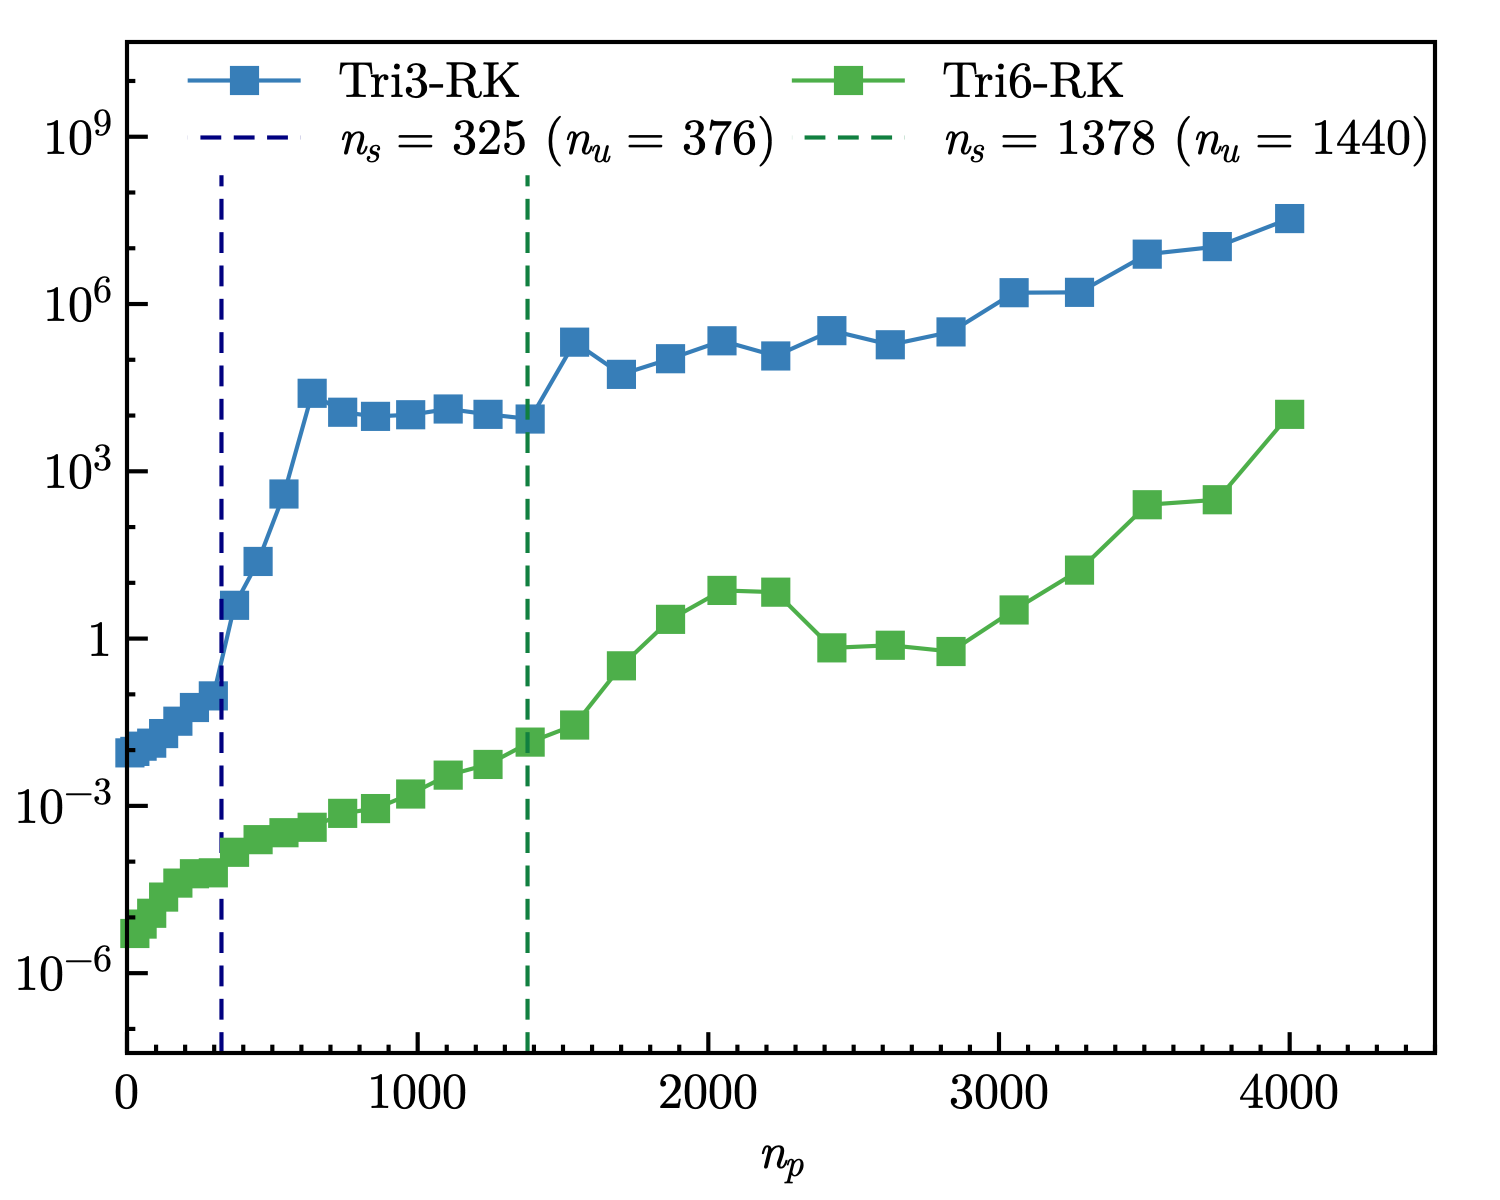
\includegraphics[width=0.48\textwidth]{png/cantilever_tri_irregular_L2_p.png}} \\
\raisebox{-0.85\height}{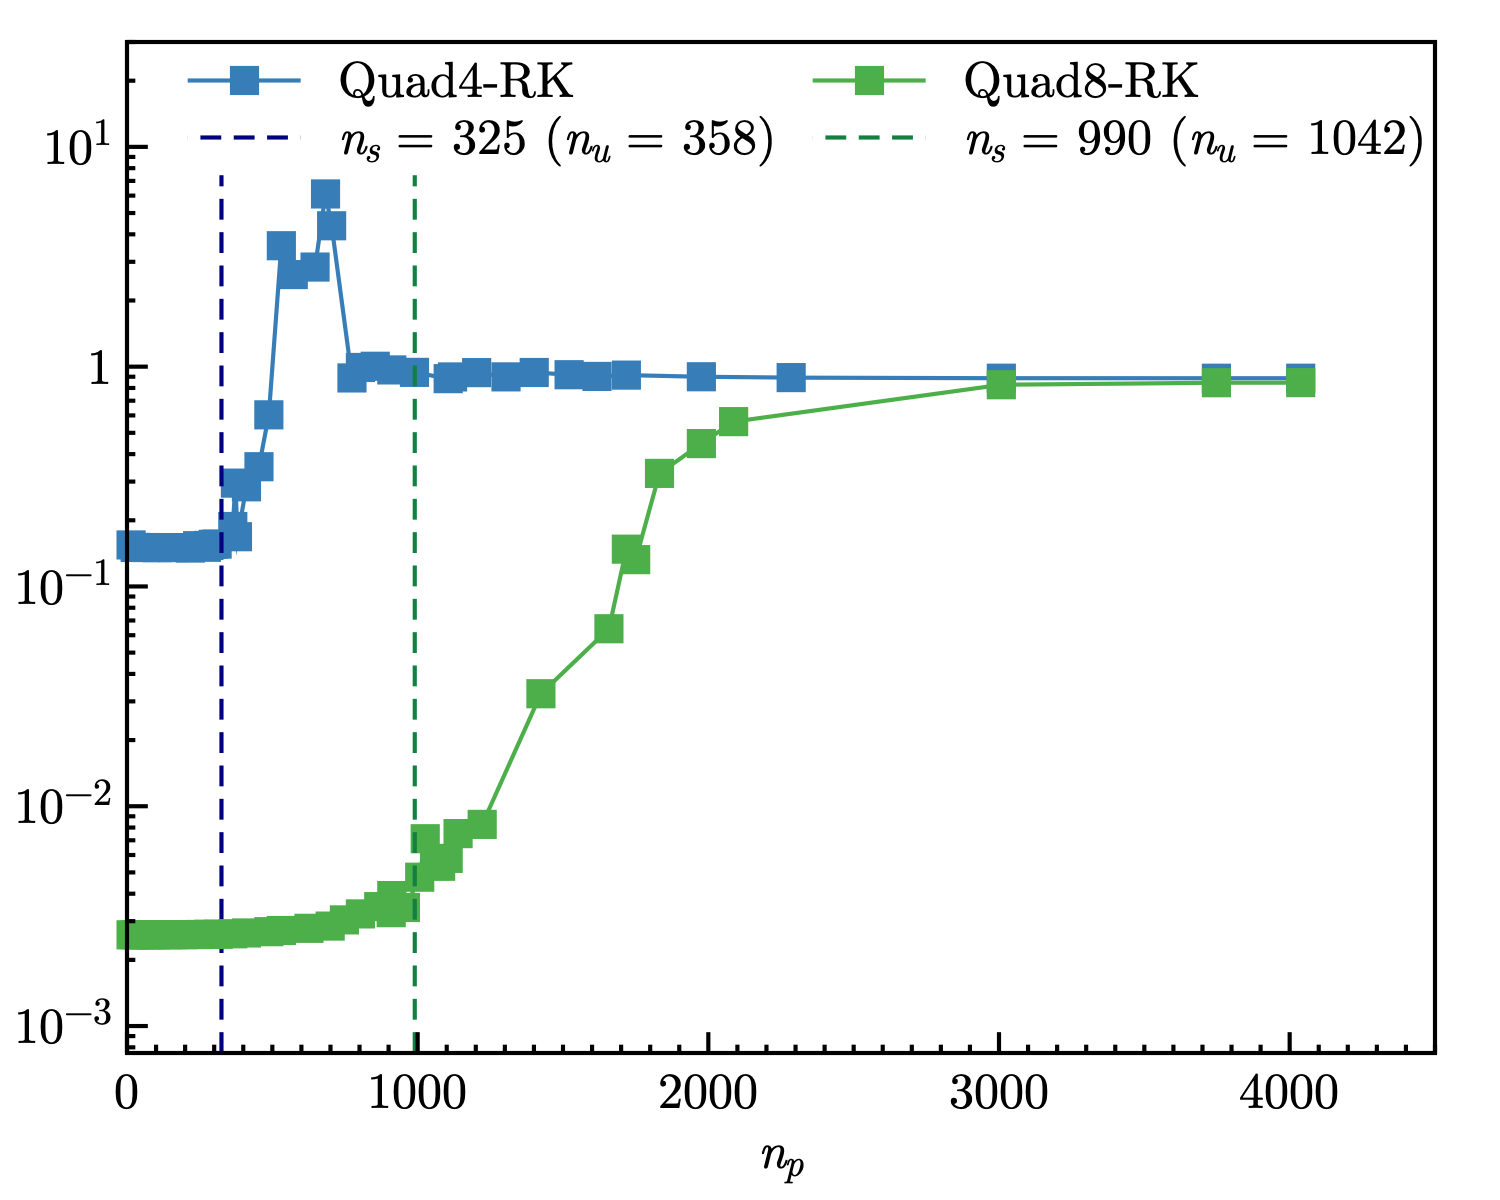
\includegraphics[width=0.48\textwidth]{png/cantilever_quad_irregular_Hdev.png}}
& \raisebox{-0.85\height}{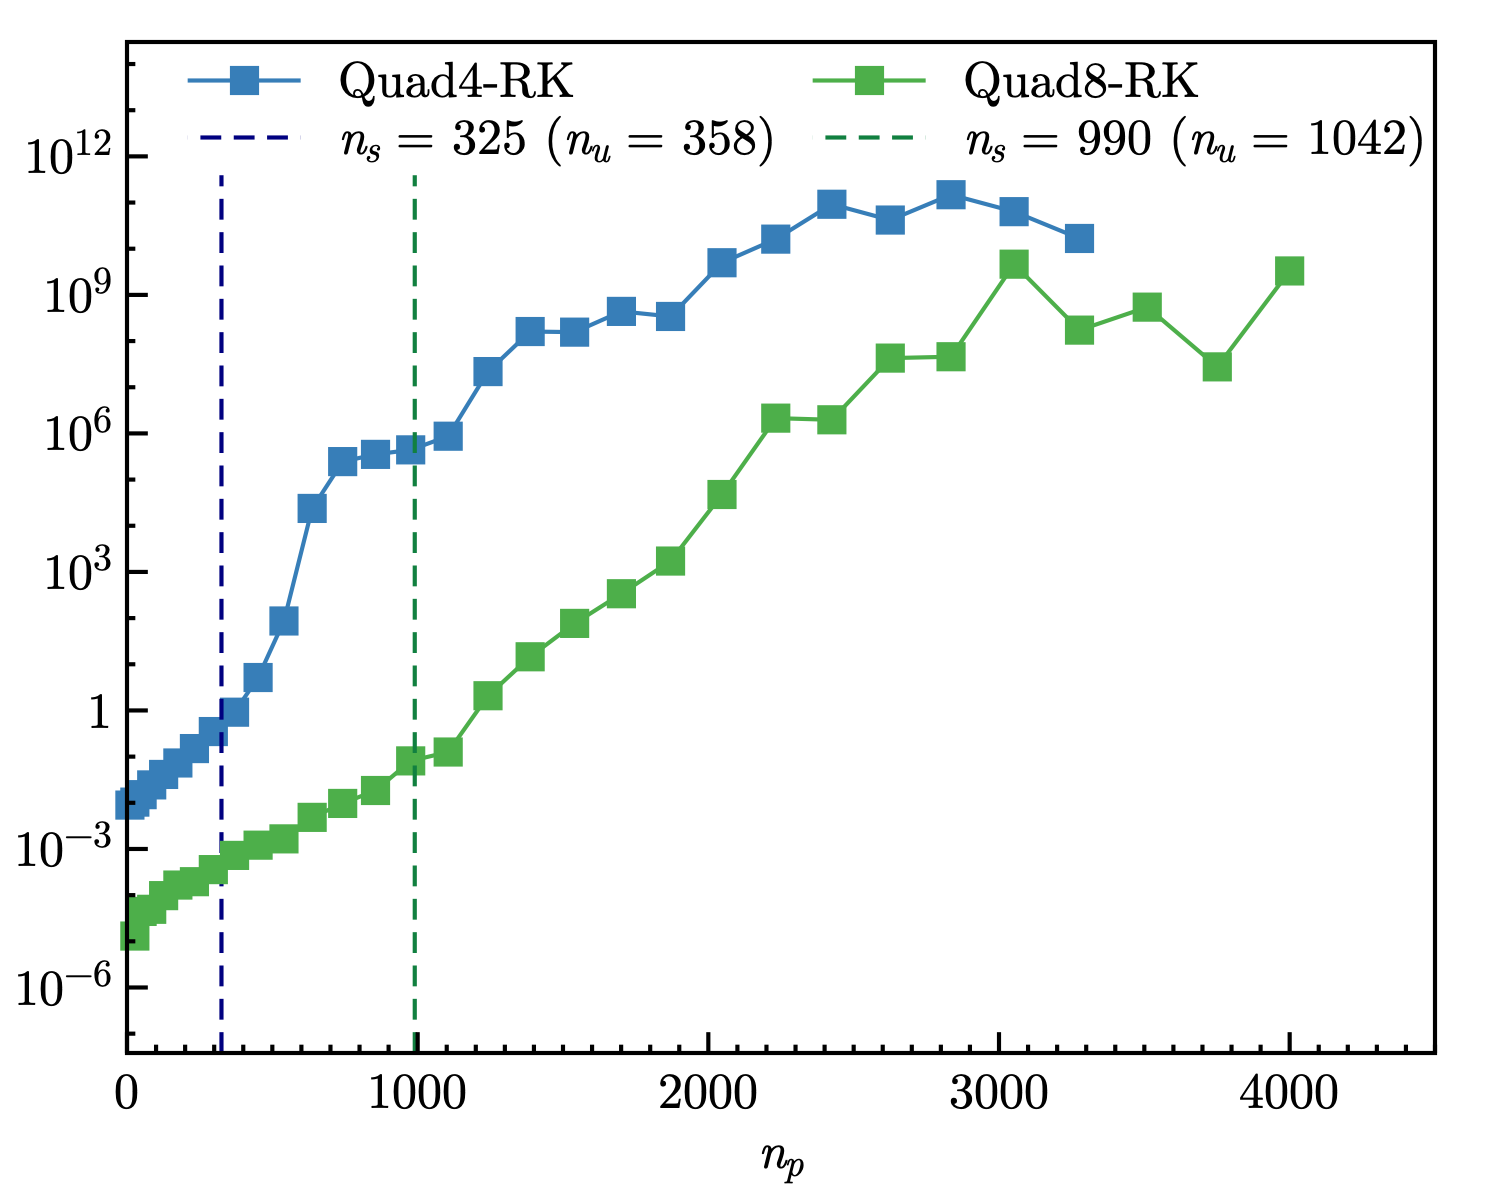
\includegraphics[width=0.48\textwidth]{png/cantilever_quad_irregularL2_p.png}} 
\end{tabular}
\end{subcaptiongroup}
\caption{Strain and pressure errors vs. $n_p$ for cantilever beam problem with non--uniform elements}\label{fg:cantilever_ns_irregular}
\end{figure}


Figures \ref{fg:cantilever_convergence_tri}, \ref{fg:cantilever_convergence} are the strain and pressure error convergence studies for triangular and quadrilateral elements, respectively,
in which Tri3--RK, Tri6--RK with $r=n_d$, the MINI element \cite{auricchio2005}, 6–-node triangular displacement element with 3–node continuous triangular pressure element (T6C3) are the comparative methods for Tri3--RK and Tri6--RK with $r=r_{opt}$,
and Quad4--RK, Quad8--RK with $r=n_d$, 4--node quadrilateral displacement element with 1--node piecewise constant pressure (Q4P1), 8--node quadrilateral displacement element with 3--node piecewise linear pressure (Q8P3) are employed for comparison with Quad4--RK and Quad8--RK with $r=r_{opt}$.
Except Tri3--RK, Quad8--RK with $r=n_d$ for strain error, all formulations with the traditional constraint ratio of $r=n_d$ cannot ensure the optimal error convergence rates. The proposed mixed formulations with $r=r_{opt}$ can maintain the optimal error convergence ratio, except the strain error of Quad8--RK is a little larger than that of Q8P3, the proposed approaches show the best performance in accuracy.

\begin{figure}[H]
\centering
\begin{subcaptiongroup}
\centering
\parbox[b]{0.49\textwidth}{
    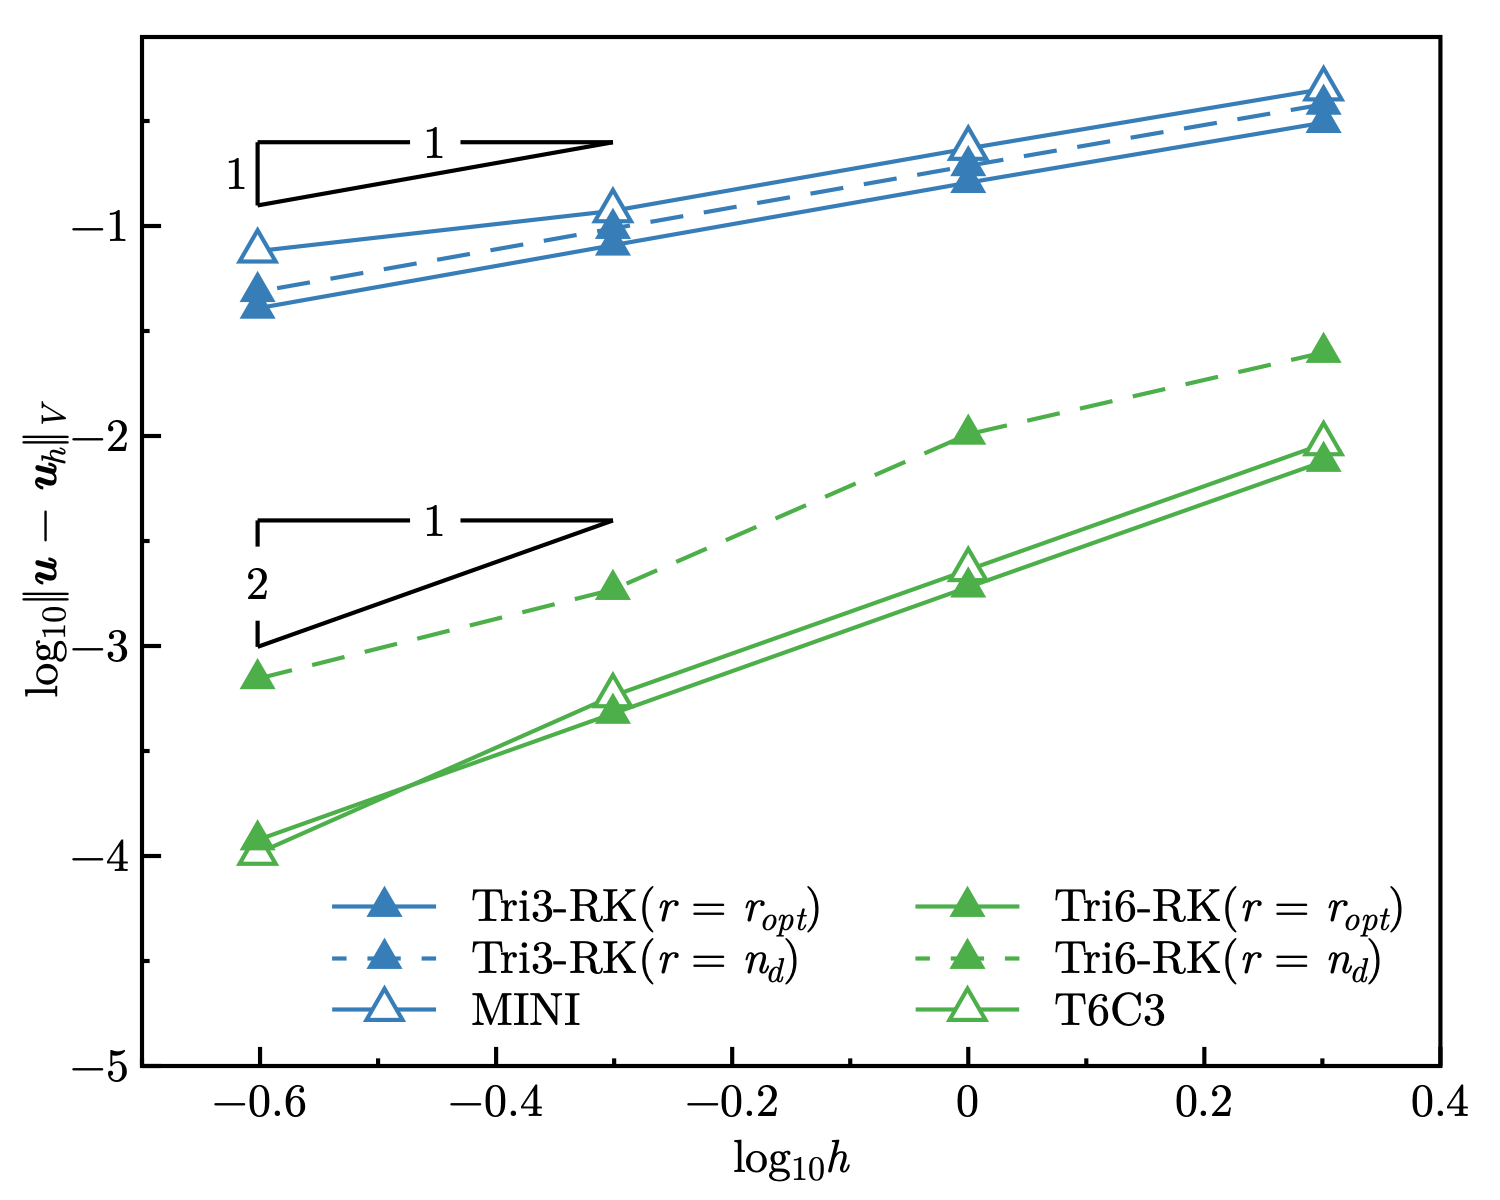
\includegraphics[width=0.49\textwidth]{png/cantilever_tri_Hdev.png}
    \caption{Strain error}\label{fg:cantilever_convergence_strain_tri}
}
\parbox[b]{0.49\textwidth}{
    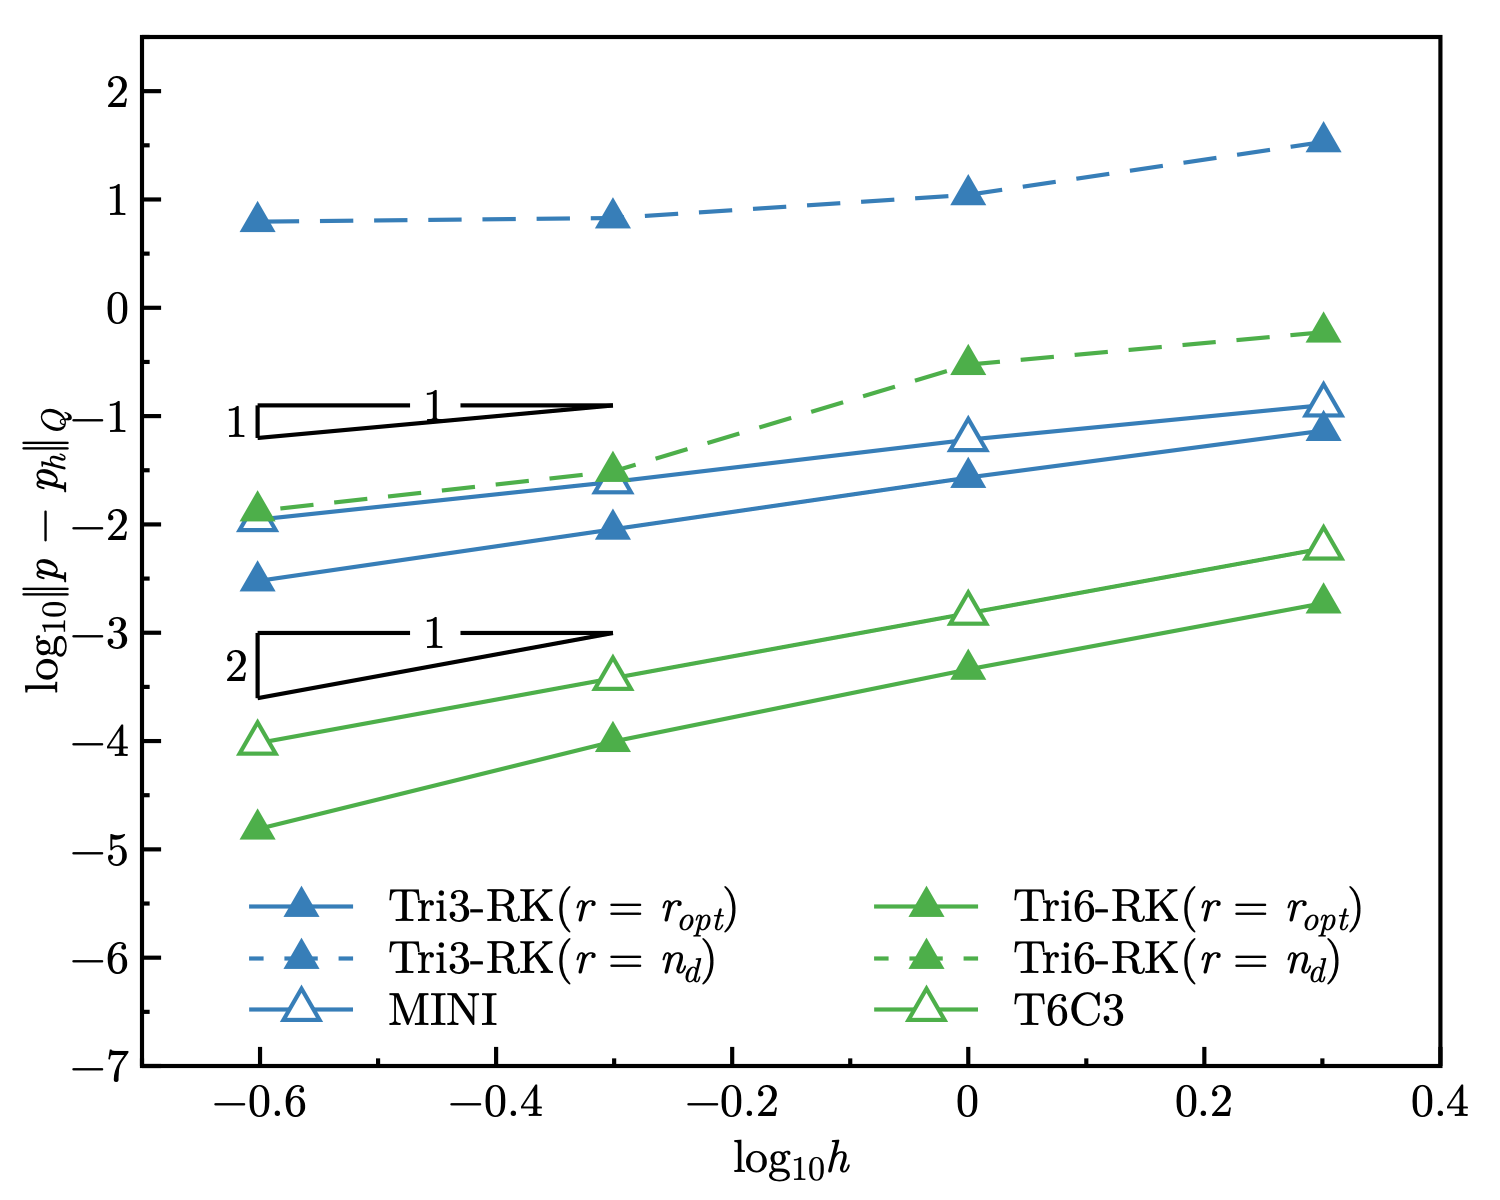
\includegraphics[width=0.49\textwidth]{png/cantilever_tri_L2_p.png}
    \caption{Pressure error}\label{fg:cantilever_convergence_pressure_tri}
}
\end{subcaptiongroup}
\caption{Error convergence study for cantilever beam problem with triangular elements}\label{fg:cantilever_convergence_tri}
\end{figure}

\begin{figure}[H]
\centering
\begin{subcaptiongroup}
\centering
\parbox[b]{0.49\textwidth}{
    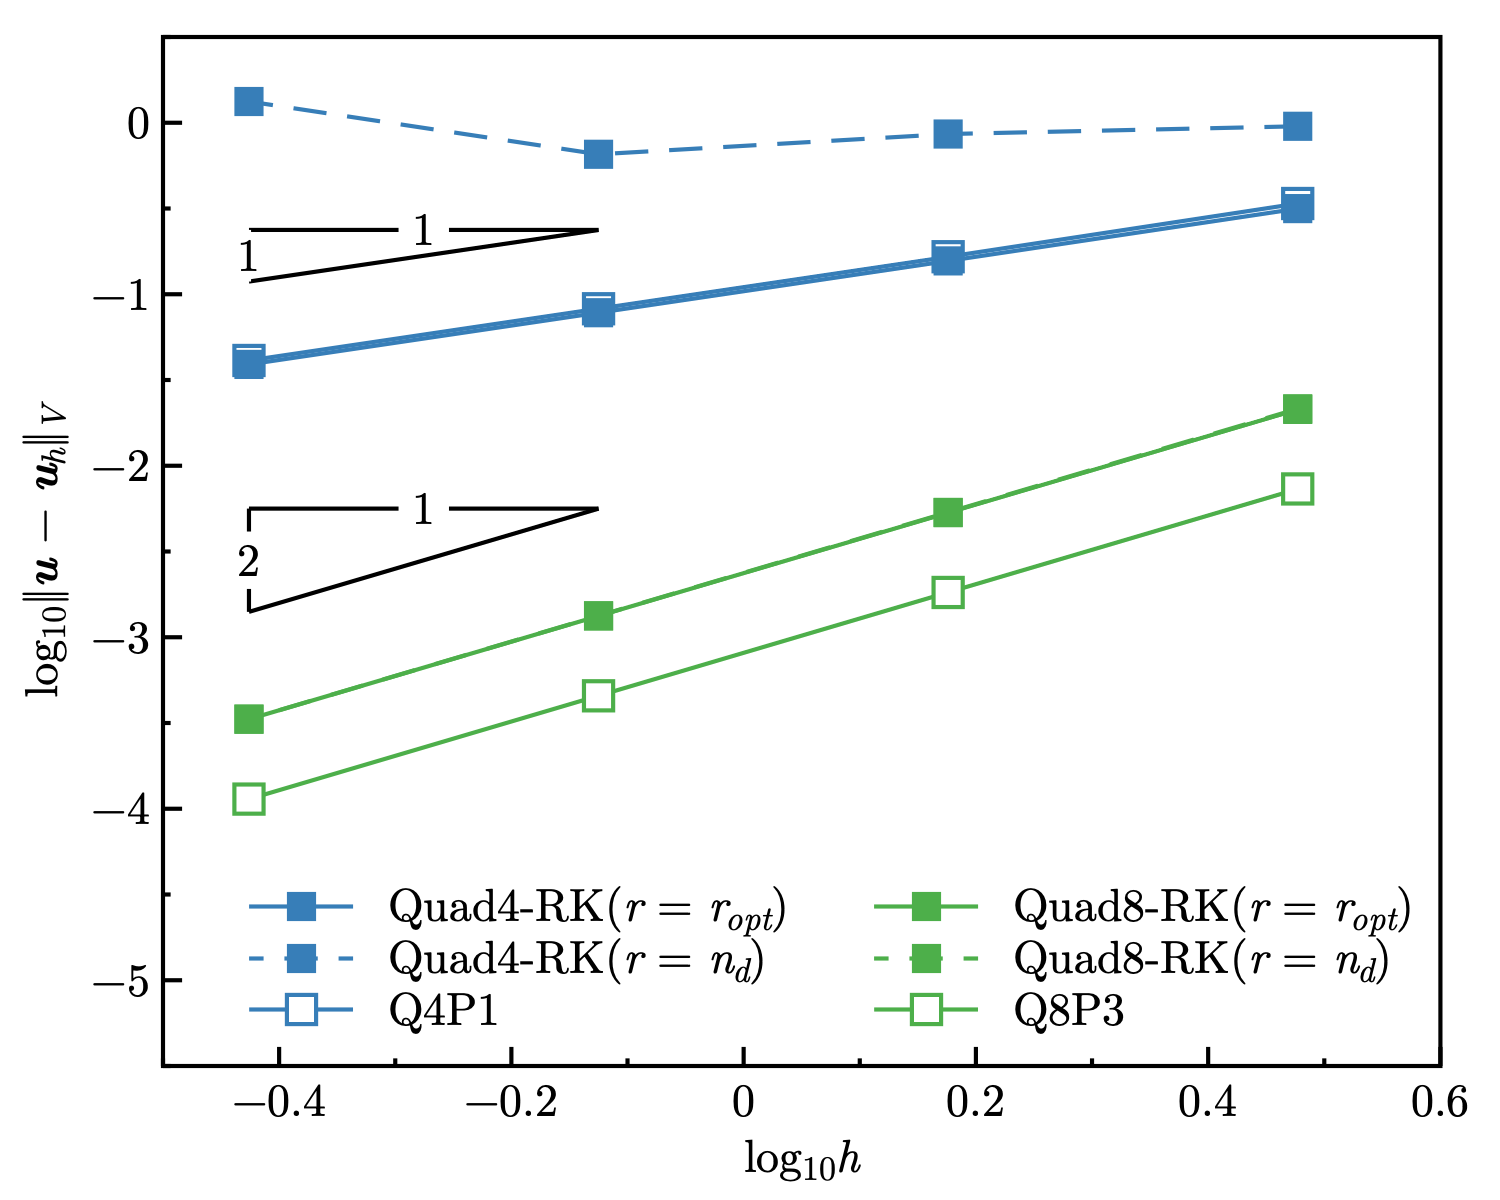
\includegraphics[width=0.49\textwidth]{png/cantilever_Hdev_r1.png}
    \caption{Strain error}\label{fg:cantilever_convergence_strain}
}
\parbox[b]{0.49\textwidth}{
    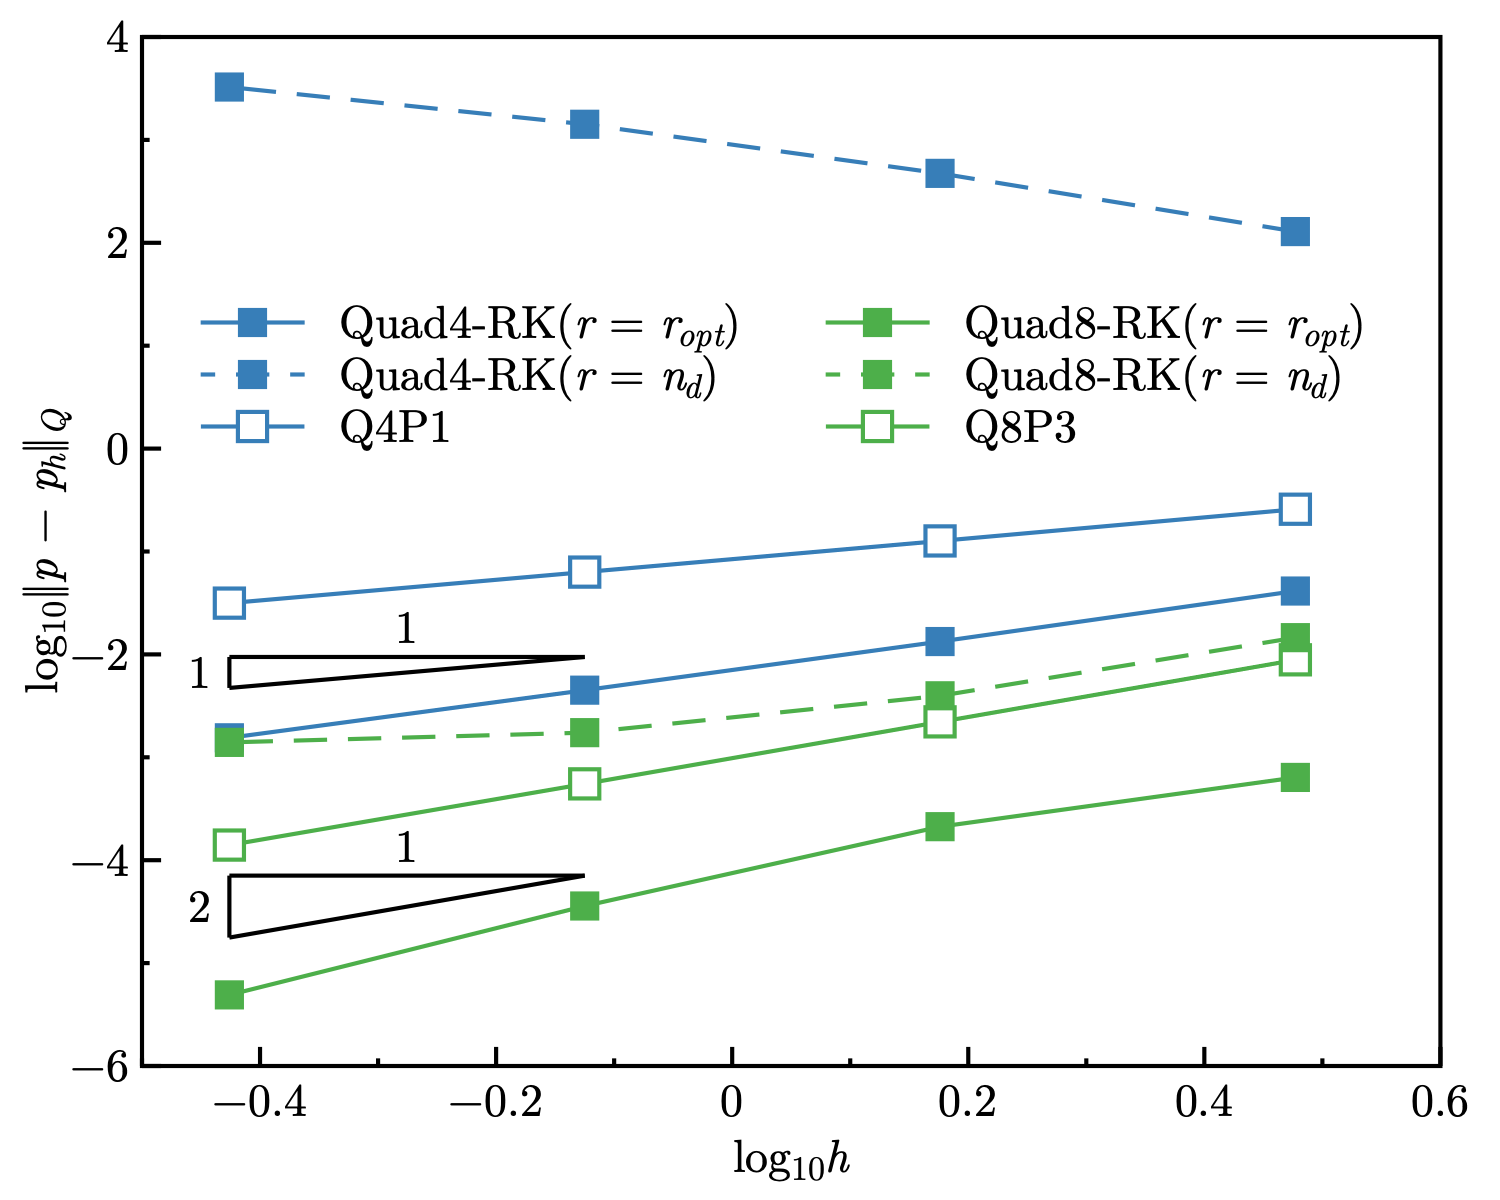
\includegraphics[width=0.49\textwidth]{png/cantilever_L2_p_r1.png}
    \caption{Pressure error}\label{fg:cantilever_convergence_pressure}
}
\end{subcaptiongroup}
\caption{Error convergence study for cantilever beam problem with quadrilateral elements}\label{fg:cantilever_convergence}
\end{figure}

